%%%%%%%%%%%%%%%%%%%%%%%%%%%%%%%%%%%%%%%%%%%%%%%
%
% Template per Elaborato di Laurea
% DISI - Dipartimento di Ingegneria e Scienza dell’Informazione
%
% update 2015-09-10
%
% Per la generazione corretta del 
% pdflatex nome_file.tex
% bibtex nome_file.aux
% pdflatex nome_file.tex
% pdflatex nome_file.tex
%
%%%%%%%%%%%%%%%%%%%%%%%%%%%%%%%%%%%%%%%%%%%%%%%

% formato FRONTE RETRO
\documentclass[epsfig,a4paper,11pt,titlepage,twoside,openany]{book}
\usepackage{epsfig}
\usepackage{plain}
\usepackage{setspace}
\usepackage[paperheight=29.7cm,paperwidth=21cm,outer=1.5cm,inner=2.5cm,top=2cm,bottom=2cm]{geometry} % per definizione layout
\usepackage{titlesec} % per formato custom dei titoli dei capitoli

%%%%%%%%%%%%%%
% supporto lettere accentate
%
%\usepackage[latin1]{inputenc} % per Windows;
\usepackage[utf8x]{inputenc} % per Linux (richiede il pacchetto unicode);
%\usepackage[applemac]{inputenc} % per Mac.

%%%%%%%%%%%%%%
% definizioni
\usepackage{amsmath}
\usepackage{amsthm}
\usepackage{amssymb}
\usepackage{mathrsfs}

%%%%%%%%%%%
% vref
\usepackage[italian]{varioref}
\usepackage{hyperref}
\hypersetup{
    colorlinks,
    citecolor=black,
    filecolor=black,
    linkcolor=black,
    urlcolor=black
}

\usepackage{url}


%%%%%%%%%%%%%%%
% algoritmi
\usepackage[ruled,linesnumbered,vlined,scleft,italiano]{algorithm2e}
\usepackage{eqparbox}
\newcommand{\algcmnt}[1]{%
  \texttt{\hfill// \eqparbox{COMMENT}{#1}}%
}
\newcommand{\alglcmnt}[1]{%
  \texttt{
    \hfill// \begin{minipage}[t]{
      \eqboxwidth{COMMENT}
    }#1\strut\end{minipage}
  }
}
\SetKwRepeat{Do}{do}{while}
% \newcommand{\forcond}{$i=0$ \KwTo $n$}
% \SetKwProg{Fn}{Function}{}{end}
% \SetKwFunction{FRecurs}{FnRecursive}%
\newcommand{\tint}{\texttt{int}}
\newcommand{\tfloat}{\texttt{float}}
\newcommand{\tbool}{\texttt{bool}}
\newcommand{\tzgen}{\textsc{ZipfGenerator}}
\newcommand{\False}{\texttt{False}}
\newcommand{\True}{\texttt{True}}

% \usepackage{algorithm}
% \usepackage{algorithmicx}
% \usepackage[noend]{algpseudocode}
% \def\NoNumber#1{{\def\alglinenumber##1{}\State #1}\addtocounter{ALG@line}{-1}}
% \floatname{algorithm}{}
\newcommand{\abracks}{[\,]}

%%%%%%%%%%%%%%%%
% tabelle
\usepackage{array}
\usepackage{multirow}
\usepackage{booktabs}
% \usepackage{caption}
\usepackage{siunitx} % formattazione numeri 
\usepackage[dvipsnames]{xcolor}
\newcommand{\1}[1]{\colorbox{Cerulean!50}{#1}}
\newcommand{\2}[1]{\colorbox{Cerulean!35}{#1}}
\newcommand{\3}[1]{\colorbox{Cerulean!20}{#1}}

%%%%%%%%%%%%%%
% immagini
\usepackage{graphicx}
\usepackage{graphics}
\usepackage{chngcntr}
\counterwithout{figure}{chapter}


%%%%%%%%%%%%%%%%
% definizioni

\theoremstyle{definition}
\newtheorem{definizione}{Definizione}
\theoremstyle{plain}
\newtheorem{teorema}{Teorema}

% \newcommand{\asd}{\href{asd}}

% definizioni
\newcommand{\infsp}{\textit{influential spreaders}}
\newcommand{\layers}{\textit{layers}}
\newcommand{\muln}{\textit{multilayer network}}
\newcommand{\mulns}{\textit{multilayer networks}}
\newcommand{\mulx}{\textit{multiplex network}}
\newcommand{\gragg}{\textit{grafo aggregato}}
\newcommand{\interc}{\textit{inter-connessioni}}
\newcommand{\spproc}{\textit{spreading process}}
\newcommand{\epprob}{\textit{epidemic probability}}
\newcommand{\crepp}{\textit{critical epidemic point}}


\singlespacing

\usepackage[italian]{babel}

\begin{document}

  % nessuna numerazione
  \pagenumbering{gobble} 
  \pagestyle{plain}

\thispagestyle{empty}

\begin{center}
  \begin{figure}[h!]
    \centerline{
\psfig{file=marchio_unitrento_colore_it_202002.eps,width=0.6\textwidth}}
  \end{figure}

  \vspace{2 cm} 

  \LARGE{Dipartimento di Ingegneria e Scienza dell’Informazione\\}

  \vspace{1 cm} 
  \Large{Corso di Laurea in\\
    % ...
    Informatica
    %Ingegneria dell'Informazione e delle Comunicazioni
    %Ingegneria dell'Informazione e Organizzazione d'Impresa
    %Ingegneria Elettronica e delle Telecomunicazioni
  }

  \vspace{2 cm} 
  \Large\textsc{Elaborato finale\\} 
  \vspace{1 cm} 
  \Huge\textsc{Influential spreaders in multilayer networks\\}
  % \Large{\it{Sottotitolo (alcune volte lungo - opzionale)}}


  \vspace{2 cm} 
  \begin{tabular*}{\textwidth}{ c @{\extracolsep{\fill}} c }
  \Large{Supervisore} & \Large{Laureando}\\
  \Large{Montresor Alberto}& \Large{Masina Gabriele}\\
  \end{tabular*}

  \vspace{2 cm} 

  \Large{Anno accademico 2019/2020}
  
\end{center}



  \clearpage
 
%%%%%%%%%%%%%%%%%%%%%%%%%%%%%%%%%%%%%%%%%%%%%%%%%%%%%%%%%%%%%%%%%%%%%%%%%%
%%%%%%%%%%%%%%%%%%%%%%%%%%%%%%%%%%%%%%%%%%%%%%%%%%%%%%%%%%%%%%%%%%%%%%%%%%
%% Nota
%%%%%%%%%%%%%%%%%%%%%%%%%%%%%%%%%%%%%%%%%%%%%%%%%%%%%%%%%%%%%%%%%%%%%%%%%%
%% Sezione Ringraziamenti opzionale
%%%%%%%%%%%%%%%%%%%%%%%%%%%%%%%%%%%%%%%%%%%%%%%%%%%%%%%%%%%%%%%%%%%%%%%%%%
%%%%%%%%%%%%%%%%%%%%%%%%%%%%%%%%%%%%%%%%%%%%%%%%%%%%%%%%%%%%%%%%%%%%%%%%%%
  \thispagestyle{empty}

\begin{center}
  {\bf \Huge Ringraziamenti}
\end{center}

\vspace{4cm}


\emph{
  ...thanks to...
}

  \clearpage
  \pagestyle{plain} % nessuna intestazione e pie pagina con numero al centro

  
  % inizio numerazione pagine in numeri arabi
  \mainmatter

%%%%%%%%%%%%%%%%%%%%%%%%%%%%%%%%%%%%%%%%%%%%%%%%%%%%%%%%%%%%%%%%%%%%%%%%%%
%%%%%%%%%%%%%%%%%%%%%%%%%%%%%%%%%%%%%%%%%%%%%%%%%%%%%%%%%%%%%%%%%%%%%%%%%%
%% Nota
%%%%%%%%%%%%%%%%%%%%%%%%%%%%%%%%%%%%%%%%%%%%%%%%%%%%%%%%%%%%%%%%%%%%%%%%%%
%% Si ricorda che il numero massimo di facciate e' 30.
%% Nel conteggio delle facciate sono incluse 
%%   indice
%%   sommario
%%   capitoli
%% Dal conteggio delle facciate sono escluse
%%   frontespizio
%%   ringraziamenti
%%   allegati    
%%%%%%%%%%%%%%%%%%%%%%%%%%%%%%%%%%%%%%%%%%%%%%%%%%%%%%%%%%%%%%%%%%%%%%%%%%
%%%%%%%%%%%%%%%%%%%%%%%%%%%%%%%%%%%%%%%%%%%%%%%%%%%%%%%%%%%%%%%%%%%%%%%%%%

    % indice
    \tableofcontents
    \clearpage
    
    
          
    % gruppo per definizione di successione capitoli senza interruzione di pagina
    \begingroup
      % nessuna interruzione di pagina tra capitoli
      % ridefinizione dei comandi di clear page
      \renewcommand{\cleardoublepage}{} 
      \renewcommand{\clearpage}{} 
      % ridefinizione del formato del titolo del capitolo
      % da formato
      %   Capitolo X
      %   Titolo capitolo
      % a formato
      %   X   Titolo capitolo
      
      \titleformat{\chapter}
        {\normalfont\Huge\bfseries}{\thechapter}{1em}{}
        
      \titlespacing*{\chapter}{0pt}{0.59in}{0.02in}
      \titlespacing*{\section}{0pt}{0.20in}{0.02in}
      \titlespacing*{\subsection}{0pt}{0.10in}{0.02in}
      
%%%%%%%%%%%%%%%%%%%%%%%%%%%%%%%%%%%%%%%%%%%%%%%%%%%%%%%%%%%%%%%%%%%%%%%%%%
%%%%%%%%%%%%%%%%%%%%%%%%%%%%%%%%%%%%%%%%%%%%%%%%%%%%%%%%%%%%%%%%%%%%%%%%%%
%% Nota
%%%%%%%%%%%%%%%%%%%%%%%%%%%%%%%%%%%%%%%%%%%%%%%%%%%%%%%%%%%%%%%%%%%%%%%%%%
%% Sommario e' un breve riassunto del lavoro svolto dove si descrive 
%% l’obiettivo, l’oggetto della tesi, le metodologie e 
%% le tecniche usate, i dati elaborati e la spiegazione delle conclusioni 
%% alle quali siete arrivati.
%% Il sommario dell’elaborato consiste al massimo di 3 pagine e deve contenere le seguenti informazioni: 
%%   contesto e motivazioni
%%   breve riassunto del problema affrontato
%%   tecniche utilizzate e/o sviluppate
%%   risultati raggiunti, sottolineando il contributo personale del laureando/a
%%%%%%%%%%%%%%%%%%%%%%%%%%%%%%%%%%%%%%%%%%%%%%%%%%%%%%%%%%%%%%%%%%%%%%%%%%
%%%%%%%%%%%%%%%%%%%%%%%%%%%%%%%%%%%%%%%%%%%%%%%%%%%%%%%%%%%%%%%%%%%%%%%%%%      
      
      %%%%%%%%%%%%%%%%%%%%%%%%%%%%%%%%
      % lista dei capitoli
      %
      % \input oppure \include
      %
      \newpage
      \chapter*{Sommario} % senza numerazione
\label{sommario}

\addcontentsline{toc}{chapter}{Sommario} % da aggiungere comunque all'indice

la diffusione di una notizia in un social network, la diffusione di un'epidemia
in una rete di contatti 
Gli influential spreaders in una rete sono quei nodi che, se infettati, 
Lorem ipsum dolor sit amet, consectetur adipiscing elit. Donec sed nunc 
orci. Aliquam nec nisl vitae sapien pulvinar dictum quis non urna. 
Suspendisse at dui a erat aliquam vestibulum. Quisque ultrices pellentesque pellentesque. 
Pellentesque egestas quam sed blandit tempus. Sed congue nec risus posuere
 euismod. Maecenas ut lacus id mauris sagittis egestas a eu dui. 
 Class aptent taciti sociosqu ad litora torquent per conubia nostra, 
 per inceptos himenaeos. Pellentesque at ultrices tellus. Ut eu purus 
 eget sem iaculis ultricies sed non lorem. Curabitur gravida dui eget ex 
 vestibulum venenatis. Phasellus gravida tellus velit, non eleifend justo 
 lobortis eget.


  Sommario è un breve riassunto del lavoro svolto dove si descrive l'obiettivo, l'oggetto della tesi, le 
metodologie e le tecniche usate, i dati elaborati e la spiegazione delle conclusioni alle quali siete arrivati.  

Il sommario dell’elaborato consiste al massimo di 3 pagine e deve contenere le seguenti informazioni:
\begin{itemize}
  \item contesto e motivazioni 
  \item breve riassunto del problema affrontato
  \item tecniche utilizzate e/o sviluppate
  \item risultati raggiunti, sottolineando il contributo personale del laureando/a
\end{itemize}




      \newpage
      \chapter{Introduzione}

Lo studio di un processo di diffusione all'interno di una rete è molto utile per comprendere le dinamiche
di diversi scenari. Tra questi, la diffusione di una notizia in una rete di contatti, di un virus in una 
società, una fake news in un social network e l'accumulo di un ritardo nelle stazioni di una rete di trasporti.

Di particolare interesse è l'individuazione dei cosiddetti \infsp, ovvero dei nodi
che, se infettati, permettono di `contagiare' una grossa parte della rete.

\section{\textit{Influential spreaders} in un grafo}

Poichè i processi di simulazione della diffusione sono computazionalmente costosi, un problema
di grande importanza è quello di individuare gli \infsp\ analizzando la topologia della rete.

Il problema è stato molto studiato nei grafi `classici', dove i nodi e gli archi che li collegano 
appartengono alla stessa rete %
\cite{kitsak:infsp}\cite{basaras:infsp}\cite{pei:infsp}.
È stato osservato che alcuni algoritmi di centralità forniscono una buona indicazione di 
quali sono i nodi più influenti nella diffusione. 
Tra questi, \textit{PageRank}, \textit{Betweenness Centrality} e \textit{k-core} sono algoritmi che richiedono una conoscenza
globale della topologia della rete, mentre per altri come Degree Centrality o $\mu$-PCI ogni nodo 
ha bisogno solo di una conoscenza locale della rete.

\section{\textit{Influential spreaders} in una multilayer network}

In molti dei problemi reali i nodi sono collegati tramite diversi tipi di interazioni, che non 
possono essere rappresentate in un grafo `classico'. 
Esempi di questo tipo sono la rete dei profili online collegati dalle loro interazioni
in diversi social networks (follow, amicizie, condivisioni, ecc.) e la rete delle stazioni di 
una città connesse da tratte di diversi mezzi di trasporto (rete ferroviaria, rete degli autobus, 
piste ciclabili, ecc.).

Strutture che permettono di rappresentare queste realtà sono le \muln, ossia reti in cui sono 
presenti differenti tipi di relazione tra i nodi. 

È stata studiata l'individuazione degli \infsp\ in questo tipo di reti, utilizzando 
algoritmi di centralità definiti su di esse.


      \newpage

      \chapter{Definizioni}

\begin{definizione}[Multilayer network] 
    \label{def:muln}
    Una \muln\ è una coppia $(\mathcal{G}, \mathcal{E} )$ dove
    $\mathcal{G} = \{G_i \mid i \in \{1, 2, \dots L\}\}$ è un insieme di grafi
    detti \layer\ dove un nodo può appartenere ad uno o più layer ed 
    $\mathcal{E} = \{E_{ij} \subseteq V_i~\times~V_j \mid i,j \in \{1, 2, \dots, L\}, i \neq j\}$
    è l'insieme delle \interc\ tra nodi appartenenti a layer differenti.
\end{definizione}
% \begin{figure}
%     \centering
%     \def\svgwidth{\columnwidth}
%     \def\svgheight{\columnwidth}
%     \input{img/mlexample.pdf_tex}
% \end{figure}
% 

\begin{definizione}
    Data una multilayer network $\mathcal{M}=(\mathcal{G}, \mathcal{E})$ 
    indichiamo con $|V|$ il numero totale di nodi, ossia la cardinalità dell'insieme $V = \bigcup\limits_{i} V_i$,
    con $N$ la somma del numero di nodi di ogni layer, ossia $N = \sum_{i}{|V_i|}$
    e con $E$ il numero totale di archi, $E = \sum_{i} |E_i| + \sum_{i \neq j} |E_{ij}|$.    
\end{definizione}

\begin{definizione}[Multiplex network] 
    \label{def:mulx}
    Una \mulx\ è un tipo di multilayer network dove le uniche inter-connessioni ammesse sono tra un 
    nodo e le sue controparti negli altri layer, ossia 
    $E_{ij} \subseteq \{ (v,v) \mid v \in {V_i \cap V_j} \} $.
\end{definizione}



\begin{definizione}[Grafo aggregato] 
    \label{def:gragg}
    Sia $\mathcal{M} = (\mathcal{G}, \mathcal{E} )$ una multilayer network. 
    Il \gragg\ derivato da $\mathcal{M}$ è il grafo 
    $G_{\mathit{agg}} = (V_{\mathit{agg}}, E_{\mathit{agg}})$  dove $V_{\mathit{agg}} = V$ ed 
    $E_{\mathit{agg}} = \biggl( \bigcup\limits_{i} E_{i} \biggr) \cup 
                    \biggl( \bigcup\limits_{i \neq j} E_{ij} \biggr)$.
\end{definizione}

\begin{figure}[h]
    \centering
    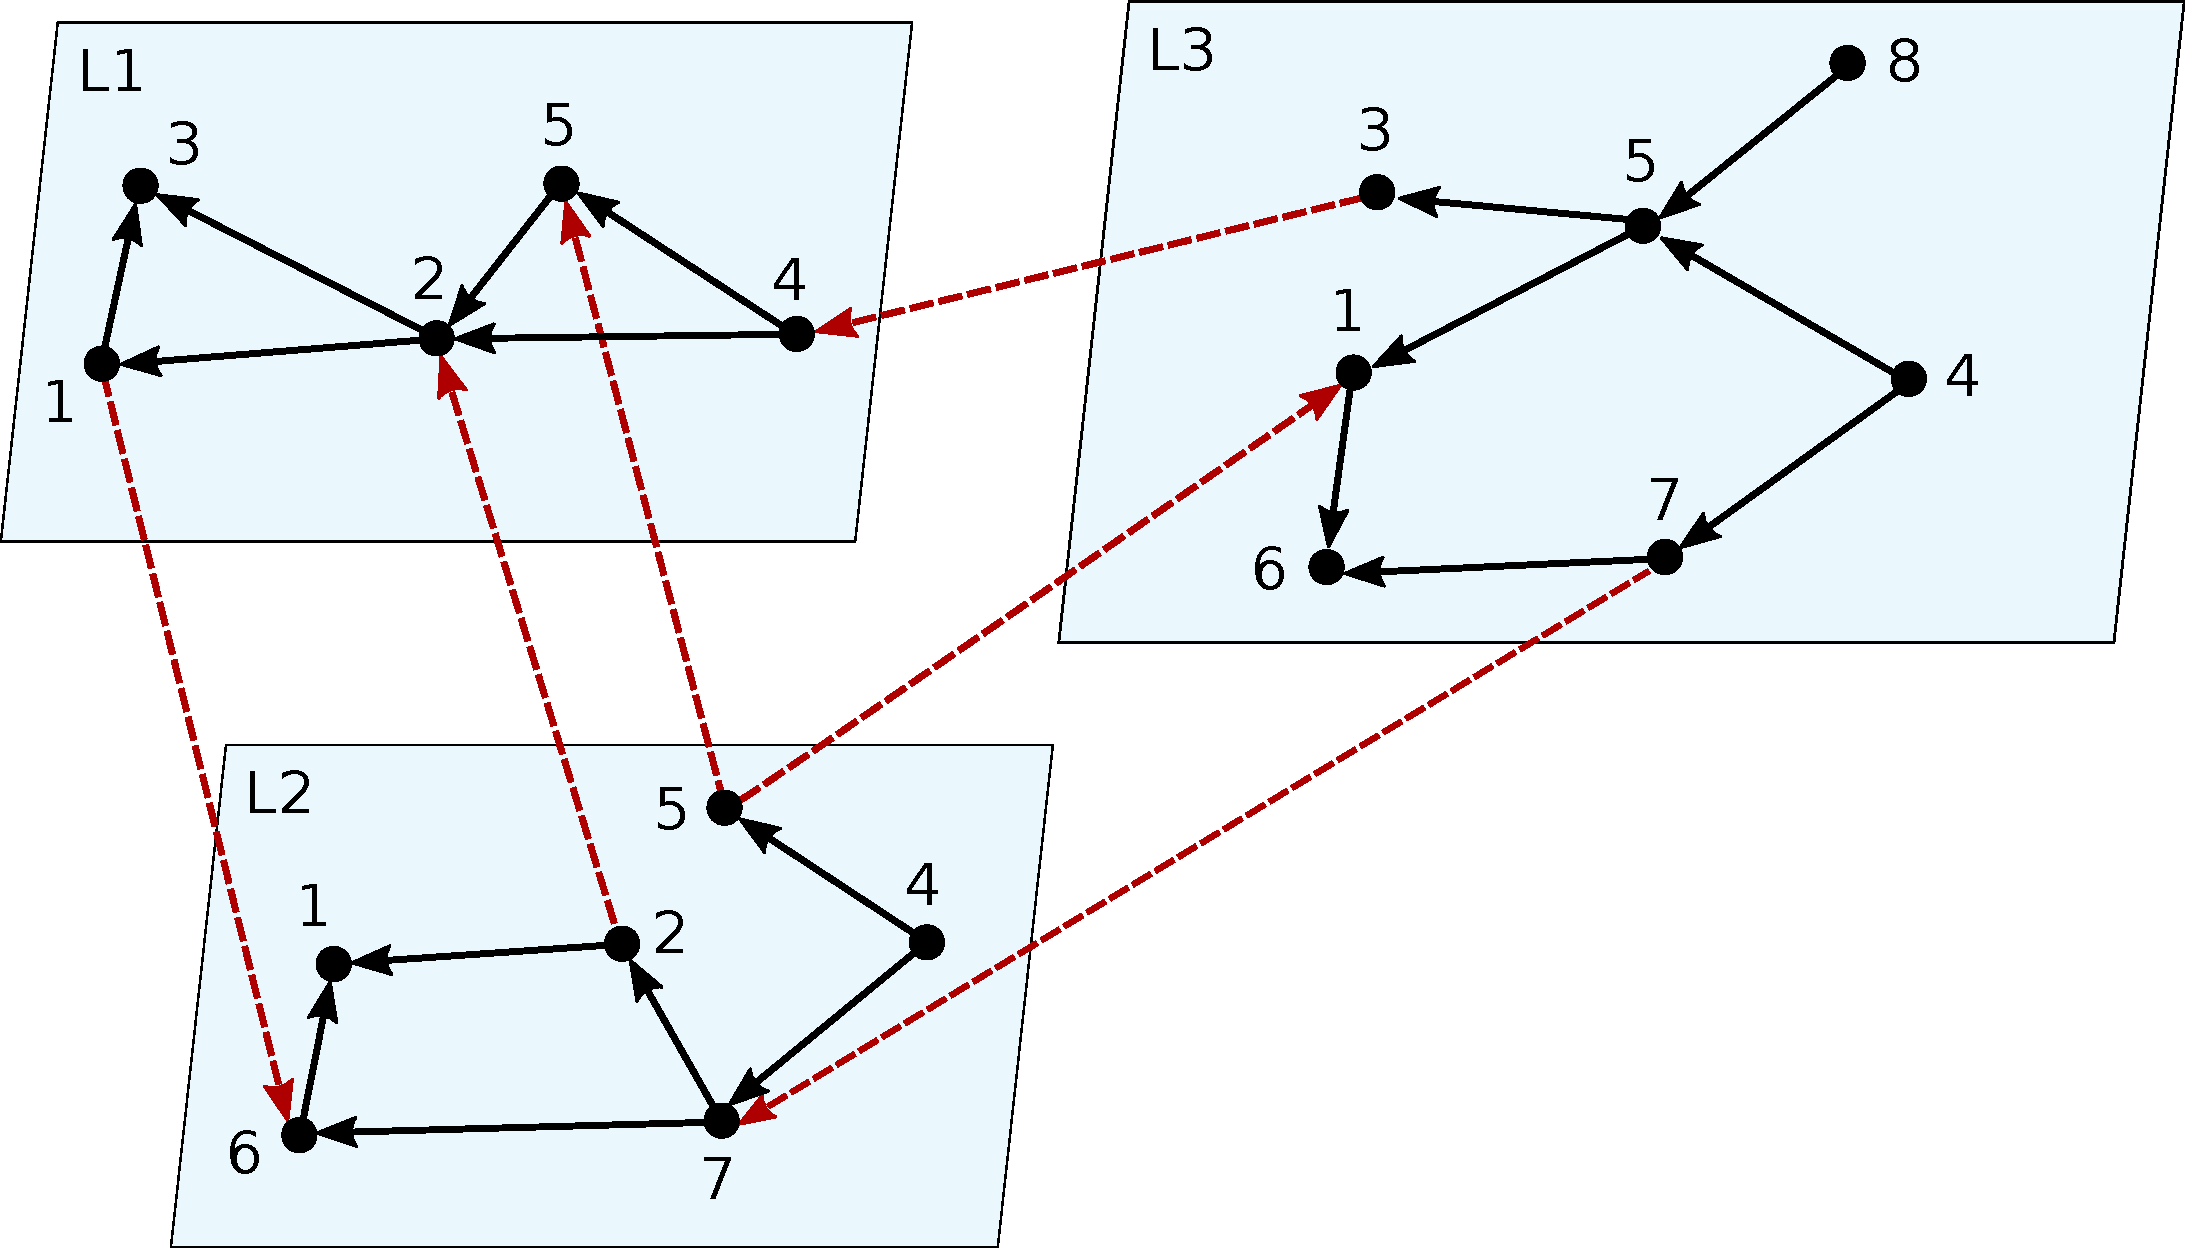
\includegraphics[height=0.3\textheight]{img/definitions/mlexample.pdf}
    \caption{Rappresentazione di una multilayer network con tre layer: L1, L2 e L3.
    In rosso sono evidenziate le inter-connessioni, ossia gli archi che collegano nodi in 
    layer differenti.}
    \label{fig:mlexample}
\end{figure}

\begin{figure}
    \centering
    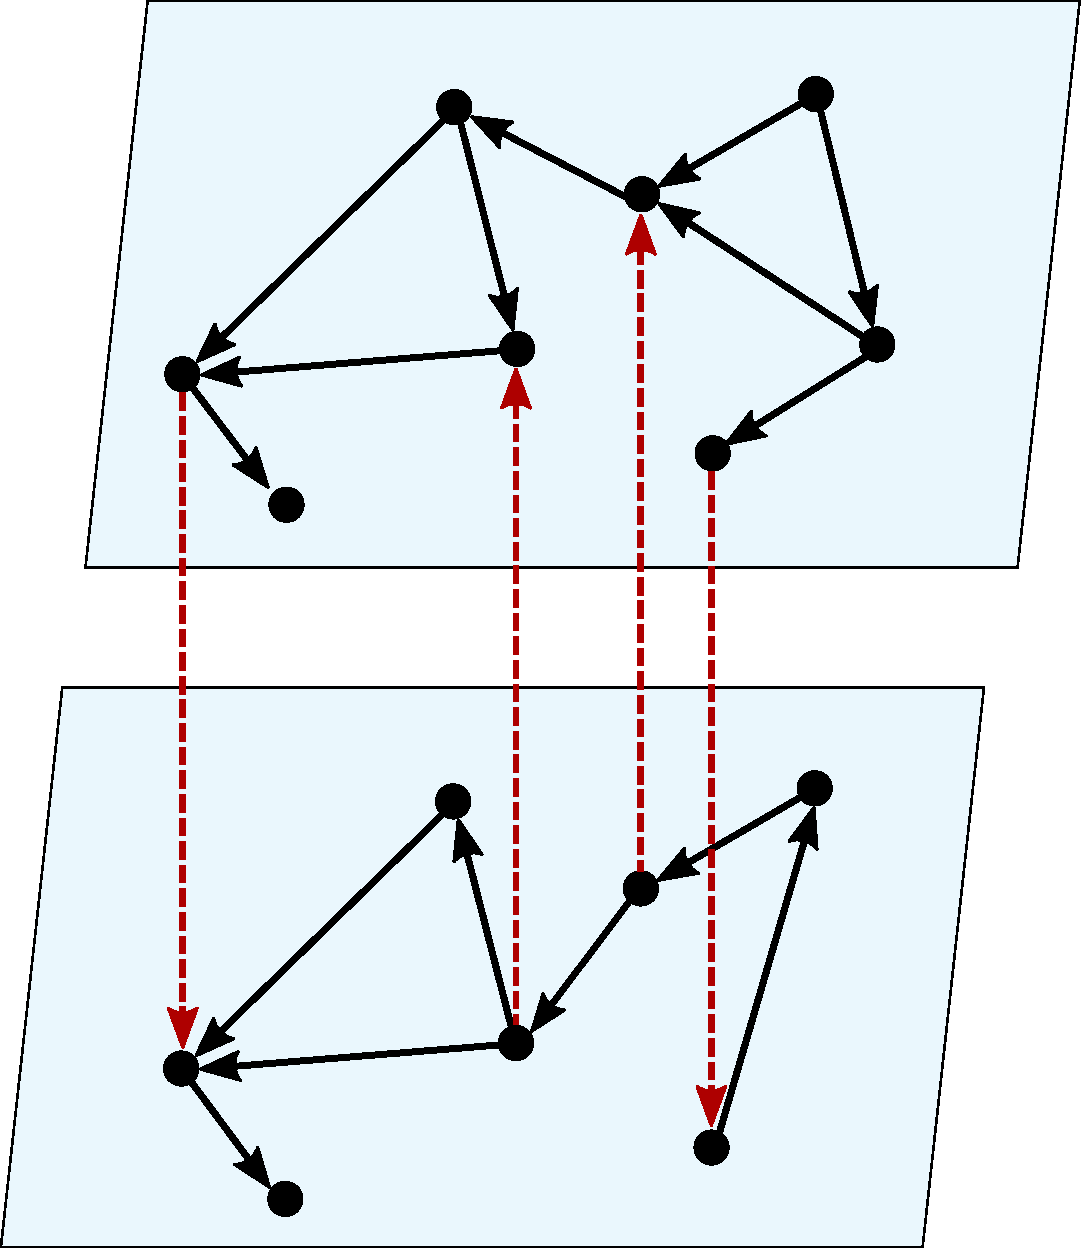
\includegraphics[height=0.3\textheight]{img/definitions/muxexample.pdf}
    \caption{Rappresentazione di una multiplex network con due layer: L1 e L2. In questo 
    tipo di rete le uniche inter-connessioni possibili sono tra un nodo e le sue controparti 
    negli altri layer.}
    \label{fig:muxexample}
\end{figure}

% 15865384615384615
\begin{figure}
    \centering
    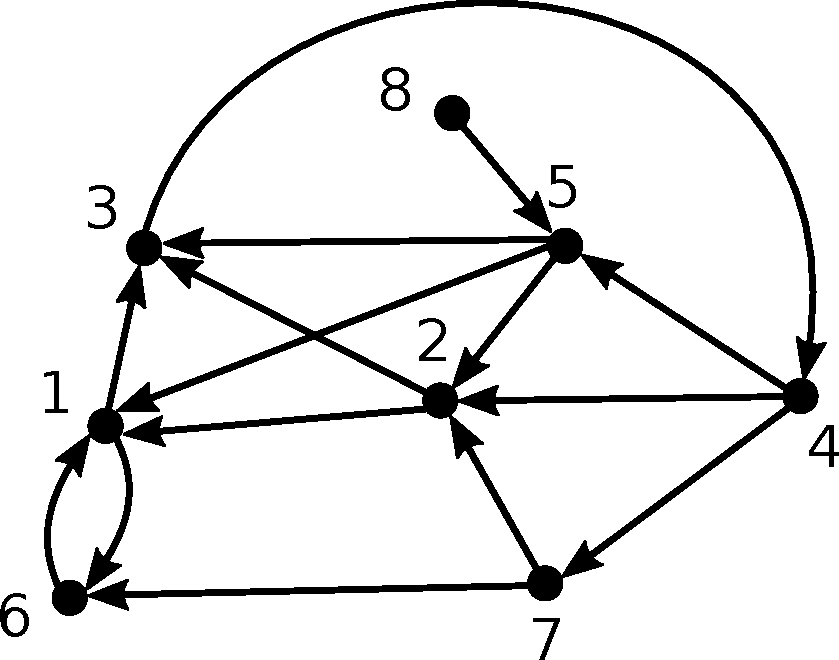
\includegraphics[height=0.15865384615384615\textheight]{img/definitions/aggexample.pdf}
    \caption{Grafo aggregato derivato dalla multilayer network rappresentata in Figura \ref{fig:mlexample}.}
    \label{fig:graggexample}
\end{figure}
%[height=0.15865384615384615\textheight]

      \newpage

      \chapter{Algoritmi utilizzati}
Dopo una fase di ricerca, sono stati selezionati ed implementati alcuni algoritmi di centralità solitamente usati per 
l'individuazione degli \infsp. Tali algoritmi assegnano ad ogni nodo un valore proporzionale alla sua centralità e 
quindi all'influenza esercitata da tale nodo sulla rete.

Questi possono essere divisi in tre categorie:
\begin{itemize}
\item algoritmi applicati sul grafo aggregato;
\item algoritmi applicati separatamente su ogni layer;
\item algoritmi applicati sull'intera struttura \textit{multilayer}.
\end{itemize}

\section{Algoritmi sul grafo aggregato}
Diverse misure di centralità sono utilizzate per identificare degli \infsp\ in grafi 
`classici' ad un solo layer, detti anche \textit{monoplex}~\cite{kitsak:infsp}\cite{basaras:infsp}\cite{pei:infsp}. 
Essendo definite per grafi ad un solo layer, sono state applicate al \gragg\
derivato da ogni \muln. 
Le misure utilizzate sono state \PageRank~\cite{page:pagerank}, 
\kcore~\cite{batagelj:kcore} e 
\degree.

% PAGE RANK

\subsection{\PageRank~(\textit{aggPR})}
\label{alg:pagerank}
\begin{definizione}[\PageRank]
    \label{def:pagerank}
    Dato un grafo $G=(V, E)$, il valore di \PageRank\ di un nodo $v$ è definito come
    \begin{equation}
        PR(v) = \alpha\sum_{w : v \in G.adj(w)}
        \frac{PR(w)}{G.outdegree(w)} + 
        (1-\alpha)\frac{1}{|V|}
    \end{equation}
    con $0 \le \alpha \le 1$.
\end{definizione}

Questa misura di centralità fu originariamente definita per misurare l'importanza di una pagina web. 
Secondo questo criterio, una pagina è tanto più importante quante più pagine importanti hanno un link 
verso di essa. 
\PageRank\ può essere visto come un modello di comportamento di un utente che, trovandosi inizialmente
in una pagina casuale, continua a visitare i link che trova, ma occasionalmente riparte da un'altra 
pagina casuale.
Il parametro $\alpha$ è detto $damping factor$ e regola la probabilità che si riparta da una pagina 
casuale ed è stato impostato a \num{0.85}.

Analogamente può essere utilizzata per misurare più genericamente l'influenza di un nodo 
in un grafo.

Questa definizione ricorsiva è stata così calcolata in modo iterativo: 

% \begin{equation}
%     \begin{split}
% PR_0(v)&= PR(v) \text{ in } X_1 \\
% addPR_l(v)&= \alpha \sum_{w : v \in X_l.adj(w)} 
%         \frac{addPR_l(w)}{X_l.outdegree(w)} + 
%         (1-\alpha)\frac{addPR_{l-1}(v)}{|V| \langle addPR_{l-1} \rangle}
%     \end{split}
% \end{equation}
\begin{equation}
    \begin{split}
PR_0(v)&= \frac{1}{n}\\
PR_i(v)&= \alpha \sum_{w : v \in G.adj(w)} 
\frac{PR_{i-1}(w)}{G.outdegree(w)} + 
(1-\alpha)\frac{1}{|V|}
    \end{split}
\end{equation}
finché $||PR_{i} - PR_{i-1}||_1 < \epsilon$. Secondo \cite{page:pagerank} il numero di iterazioni 
è proporzionale a $\log{|V|}$. Dunque, la complessità dell'algoritmo è $O((|V| + |E|)\log{|V|})$.

% K-CORE

\subsection{\kcore~(\textit{aggCore})}
\begin{definizione}[\kcore]
    \label{def:kcore}
    Dato un grafo $G=(V, E)$, un \kcore\ di $G$ è un sottografo $G'=(V',E')$
    tale che 
    \begin{equation}
        G'.indegree(v) \geq k \quad \forall v \in V'
    \end{equation}
\end{definizione}

Un nodo appartenente ad un \textit{k-core} con $k$ elevato è considerato un nodo centrale 
nella rete, e quindi un potenziale \textit{influential spreader}.
Per il calcolo di questa misura è stato utilizzato l'algoritmo definito in~\cite{batagelj:kcore}
con complessità $O(|V| + |E|)$.

\subsection{\degree~(\textit{aggDeg})}
Questa misura di centralità assegna ad ogni nodo un valore pari al suo \textit{outdegree}, 
per cui un nodo con tanti vicini si assume possa avere una certa rilevanza in un 
processo di diffusione.
Può essere calcolata con complessità $O(|V|)$.

\section{Algoritmi applicati su ogni layer}
Alcune delle misure sono state estese alle reti multilayer calcolando la centralità
dei nodi in ogni layer separatamente e poi sommando i punteggi ottenuti in ogni layer.
In questa categoria rientrano \addPageRank~\cite{halu:addpagerank} 
e \sumCore~\cite{basaras:infspmul}

\subsection{\addPageRank~(\textit{addPR})}
\begin{definizione}[\addPageRank]
    Data una \muln\ $\mathcal{M}=(\mathcal{G}, \mathcal{E})$ 
    ed un ordinamento dei layer $(X_1, \dots, X_{L})$, l'\addPageRank\
    di un nodo $v \in V$ è il valore 
    $addPR(v) = addPR_L(v)$, dove:

    \begin{equation}
        \begin{split}
addPR_1(v)&= PR(v) \text{ in } X_1 \\
addPR_l(v)&= \alpha \sum_{w : v \in X_l.adj(w)} 
            \frac{addPR_l(w)}{X_l.outdegree(w)} + 
            (1-\alpha)\frac{addPR_{l-1}(v)}{|V| \langle addPR_{l-1} \rangle}
        \end{split}
    \end{equation}

\end{definizione}

Questa estensione dell'algoritmo di PageRank alle \muln\ richiede un ordinamento
dei layer. Come fatto in \cite{basaras:infspmul}, i layer sono stati ordinati per valore
dell'autovalore di modulo massimo della rispettiva matrice di adiacenza. Infatti, 
autovalore più grande significa maggiore capacità di diffusione~\cite{wang:eigenv}.

Come algoritmo, è stato utilizzato un approccio analogo a quello della versione classica di 
PageRank descritto in~\vref{alg:pagerank}.
Poiché è necessario calcolare il PageRank su ogni layer, il costo dell'algoritmo è 
$O(\sum_{i}((|V_i| + |E_i|)log(|V_i|)))$, assumendo che i layer siano già ordinati.

\subsection{\sumCore~(\textit{sumCore})}
Questa misura è stata ottenuta calcolando il valore di \kcore di ogni nodo in 
ogni layer, quindi sommando i valori ottenuti da un nodo in tutti i layer.
Pertanto la complessità del calcolo è pari a $O(\sum_{i}(|V_i| + |E_i|)$.

\section{Algoritmi applicati sull'intera struttura}
Diverse misure definite originariamente per grafi \textit{monoplex} sono state estese a 
reti \textit{multilayer}. Queste, al contrario di quelle presentate nelle sezioni precedenti,
tengono conto della struttura a più livelli della rete ed in particolare delle \interc.
Quelle implementate sono 
\verPageRank~\cite{dedomenico:versatile},
\verBetweennessCentrality~\cite{dedomenico:versatile} \cite{dedomenico:verbetw},
\multiCore~\cite{azimi:multikcore} e le diverse varianti di \PCI: 
\mlPCI~\cite{basaras:infspmul},
\laPCI~\cite{basaras:infspmul},
\alPCI~\cite{basaras:infspmul},
\lsPCI~\cite{basaras:infspmul}.

\subsection{\verPageRank~(\textit{verPR})}
\begin{definizione}[\verPageRank]
    Data una \muln\ $\mathcal{M}=(\mathcal{G}, \mathcal{E})$,
    si definisce \verPageRank\ di un nodo $v \in V_l$ in un layer $l$
    il valore:

    \begin{equation}
        PR(v, l) = 
        \alpha \biggl( 
            \sum_{w : v \in G_l.adj(w)} \frac{PR(w, l)}{\mathcal{M}.outdegree(w, l)} +
            \sum_{j \neq l}^{}\sum_{w : (w, v) \in E_{jl}} \frac{PR(w, j)}{\mathcal{M}.outdegree(w, j)} 
        \biggr) + (1-\alpha)\frac{1}{N}
    \end{equation}
    dove $\mathcal{M}.outdegree(w, l)$ è la somma del numero di archi uscenti da $w$ nel layer $l$
    e del numero di \interc\ uscenti da $w$ nel layer $l$.

\end{definizione}

La definizione originale in \cite{dedomenico:versatile} utilizzava un tensore 4-dimensionale per 
rappresentare la rete. Qui è stata generalizzata, anche prevedendo che un nodo possa non comparire 
in tutti i layer.

Questa definizione è stata calcolata in modo analogo alla definizione \vref{alg:pagerank},
dunque la complessità è $O((N + E)\log(N))$.

\subsection{\verBetweennessCentrality~(\textit{verBC})}

\begin{definizione}[\verBetweennessCentrality]
    Data una \muln\ $\mathcal{M}=(\mathcal{G}, \mathcal{E})$, la 
    \verBetweennessCentrality\ di un nodo $v$ è il valore 
    \begin{equation}
        BC(v) = \sum_{s, t \in V} \frac{\sigma_{st}(v)}{\sigma_{st}}
    \end{equation}
    dove $\sigma_{st}$ è il numero di percorsi minimi tra il nodo $s$ ed il nodo $t$
    indipendentemente dal layer, e $\sigma_{st}(v)$ è il numero di questi che passa 
    per il nodo $v$ in qualche layer.
\end{definizione}

Questa misura è stata calcolata con l'algoritmo definito in \cite{dedomenico:verbetw}, 
con complessità $O\left(|V|\left(N+E\right)\right)$.

\subsection{\multiCore~(\textit{multiCore})}

\begin{definizione}[\multiCore]
    Data una \muln\ $\mathcal{M}=(\mathcal{G}, \mathcal{E})$, il \multiCore\ è
    il più grande sottografo per cui ogni nodo è raggiunto in ogni layer da almeno $k$ archi o
    \interc.
\end{definizione}

Questa misura è stata calcolata estendendo l'algoritmo definito in \cite{batagelj:kcore} per 
adattarlo a questa definizione, ottenendo una complessità di $O(N + E)$.

\subsection{\PCI~(\textit{PCI})}
\begin{definizione}
    Data una \muln\ $\mathcal{M}=(\mathcal{G}, \mathcal{E})$, 
    l'indice $mlPCI_n$ di un nodo $v$ in un layer $l$ 
    è il massimo numero $k$ tale che esistono almeno $k$ vicini di $v$ nel layer $l$ in $\mathcal{M}$
    con numero di vicini in almeno $n$ layer maggiore o uguale a $k$.
\end{definizione}

Da questa definizione si ricavano le seguenti:

\begin{definizione}[\mlPCI]
    L'indice $mlPCI$ di un nodo $v$ in un layer $l$ è definito come 
    \begin{equation}
        mlPCI(v, l) = \sum_{n=1}^L mlPCI_n(v, l)
    \end{equation}
\end{definizione}

\begin{definizione}[\alPCI]
    L'indice $alPCI$ di un nodo $v$ in un layer $l$ è definito come 
    \begin{equation}
        alPCI(v, l) = mlPCI_L(v, l)
    \end{equation}
\end{definizione}


\begin{definizione}[\lsPCI]
    L'indice $lsPCI$ di un nodo $v$ in un layer $l$ è il massimo numero $k$ 
    tale che esistono almeno $k$ vicini di $v$ nel layer $l$ in $\mathcal{M}$
    con numero di vicini in almeno $k$ layer maggiore o uguale a $k$.
\end{definizione}

\begin{definizione}[\laPCI]
    L'indice $laPCI$ di un nodo $v$ in un layer $l$ è 
    è il massimo numero $k$ tale che esistono almeno $k$ vicini di $v$ nel layer 
    $l$ in $\mathcal{M}$
    con numero di vicini maggiore o uguale a $k$.
\end{definizione}



Il calcolo di queste definizioni, è stato fatto utilizzando un algoritmo di complessità 
$O(N L t \log{t})$, dove $t = \max{\{\mathcal{M}.outdegree(v)\,|\,v \in V\}}$ 

      \newpage
      
      \chapter{Dataset}
Queste misure sono state testate su diverse reti con caratteristiche diverse, 
seguendo una metodologia simile a \cite{basaras:infspmul}:
\begin{itemize}
    \item Multiplex Network estratte da dataset biologici e sociali;
    \item Multilayer Network generate a partire da reti di interazioni in Internet.
\end{itemize}

\section{Estrazione reti multiplex}
Le reti indicate in tabella \vref{tab:multiplex} sono state estratte a partire da reti biologiche e
sociali fornite da \cite{data:multiplex}.
L'obiettivo era quello di ottenere un dataset simile a quello utilizzato da \cite{basaras:infspmul},
dove per ogni rete sono indicati i numeri $N$, $E$ ed $|L|$, rispettivamente di nodi, archi e layer estratti.

Per ogni rete, è stato individuato un sottoinsieme $L$ di $|L|$ layer in cui il numero di nodi con una 
controparte in ogni layer fosse almeno $N$. Per tutte le reti, è  stato trovato un solo sottoinsieme 
che rispettasse questo criterio.

Dopo aver costruito una sotto-rete formata solo dai layer in $L$, sono stati rimossi i nodi non presenti
in tutti i layer e gli archi da e verso essi. Dopodichè sono stati rimossi tutti i nodi da cui non arrivava
nè partiva più nessun arco. Questa procedura è stata applicata ricorsivamente alla sotto-rete ottenuta, 
finchè non è stato più possibile rimuovere alcun nodo. 

I risultati ottenuti sono stati molto simili a quelli voluti, come si può vedere in tabella \vref{tab:multiplex}.

In queste reti sono state aggiunte \interc\ tra le controparti di ogni nodo in ogni layer.


% reti multiplex 

\begin{table}
    \caption{Multiplex network estratte}
    \label{tab:multiplex}
    \centering
    \begin{tabular}{lrrrrrrrr}
        \toprule
              \multirow{2}*{Nome} 
            & \multicolumn{3}{c}{Nodi} 
            & \multicolumn{3}{c}{Archi} 
            & \multicolumn{2}{c}{Layers} \\
            \cmidrule(lr){2-4} \cmidrule(lr){5-7} \cmidrule(lr){8-9}                    
            
            
            & iniziali & obiettivo & estratti 
            & iniziali & obiettivo & estratti 
            & iniziali & estratti \\
            
            % Nodi iniziali & Nodi estratti in  & Nodi estratti & Archi iniziali & Archi estratti in  & Archi estratti & Layer iniziali & Layer estratti \\
        \midrule
            Drosophila          & \num{  8215} & \num{  1364} & \num{1375}
                                & \num{ 43366} & \num{  7267} & \num{7438} 
                                & \num{     7} & \num{     2} \\
            Homo                & \num{ 18222} & \num{  3859} & \num{3878}
                                & \num{170899} & \num{ 77483} & \num{78804} 
                                & \num{     7} & \num{     3} \\
            MA2013              & \num{ 88804} & \num{  4370} & \num{4377}
                                & \num{210250} & \num{ 33411} & \num{34589} 
                                & \num{     3} & \num{     3} \\
            NYCM2014            & \num{102439} & \num{  4150} & \num{4262}
                                & \num{353495} & \num{ 45334} & \num{47840} 
                                & \num{     3} & \num{     3} \\
            SacchCere           & \num{  6570} & \num{  3096} & \num{3121}
                                & \num{ 28275} & \num{185849} & \num{188182} 
                                & \num{     7} & \num{     5} \\
            SacchPomb           & \num{  4092} & \num{   875} & \num{878}
                                & \num{ 63676} & \num{ 18214} & \num{ 18308} 
                                & \num{     7} & \num{     3} \\
        \bottomrule
    \end{tabular}
%         
    
\end{table}

\section{Generazione reti multilayer}
Sono state generate delle \muln\ partendo da grafi di interazioni su 
social network e su architetture peer-to-peer, in particolare quelli 
indicati in tabella \vref{tab:multilayer}, che si possono trovare in \cite{data:multilayer}.

Seguendo l'approccio di \cite{basaras:infspmul}, sono stati generati due tipi di reti:
\begin{itemize}
    \item Similar Layers Network(SLN), i cui layer sono i grafi [3-6] della  
            tabella \vref{tab:multilayer}. In queste reti i layer hanno tutti un numero simile 
            di nodi e archi;
    \item Different Layers Networks(DLN), i cui layer sono i grafi [1-3] della tabella 
        \vref{tab:multilayer}. In queste reti i layer hanno numero di nodi e archi molto differenti.
\end{itemize}

\paragraph{Generazione delle \interc}
Per prima cosa, sono state aggiunte \interc\ tra le controparti di ogni nodo in tutti 
i layer in cui esso è presente.

Quindi, sono state generate casualmente altre \interc\ impostando tre parametri:
\begin{enumerate}
    \item il numero di \interc\ uscenti da un nodo in un determinato layer;
    \item la frequenza con cui un layer viene scelto come layer di destinazione di 
        una connessione;
    \item la frequenza con cui un nodo in un certo layer viene scelto come nodo 
        di destinazione. 
\end{enumerate}
Ognuno di questi parametri è stato generato secondo una distribuzione che segue 
la legge di Zipf \cite{zipf:humanb}, per cui la frequenza di un certo valore è inversamente
proporzionale al valore stesso. 

Tale distribuzione genera numeri tra 1 ed un valore massimo $m$ con diverse probabilità,
secondo il valore di una variabile $s \in [0, 1]$
che regola il grado di `asimmetria' dei valori generati:
per $s=0$ la probabilità di ogni valore è la stessa, mentre per  
$s=1$, si ha $\mathcal{P}(1) = 2 \cdot \mathcal{P}(2) = 3 \cdot \mathcal{P}(3) =\dots = m \cdot \mathcal{P}(m)$. 

Le variabili che regolano i tre parametri sono chiamate rispettivamete
$s_{degree}$, $s_{layer}$, $s_{node}$.
Per ognuna sono stati sperimentati i valori $0.3$ e $0.8$. 
Per quanto riguarda il numero di \interc\ di un nodo in un determinato layer
il valore massimo è stato impostato a $d \cdot \log_2{\sum_{i}{V_i}}$, con 
$d = 2$. Per gli altri paramentri, invece, tutti i layer devono essere selezionabili
così come tutti i nodi all'interno di un layer.

La probabilità che un nodo abbia $k$ \interc\ è $\mathcal{P}_{degree}(k)$.
Per la scelta del layer di destinazione si è operato come segue:
è stata generata una permutazione casuale dei layer; definita $pos(l)$
la posizione del layer $l$ nella permutazione, la probabilità che questo venga 
scelto come layer di destinazione è $\mathcal{P}_{layer}(pos(l))$.
In modo analogo sono stati permutati i nodi all'interno di ogni layer per determinarne 
la probabilità di essere scelti come destinazione.

Le reti così generate sono denominate con 
SLN\large{$_{ s_{degree}\text{,}s_{layer}\text{,}s_{node}}$}
oppure
DLN\large{$_{ s_{degree}\text{,}s_{layer}\text{,}s_{node}}$}

L'algoritmo \vref{alg:generate} mostra come sono state generate le reti.

\SetStartEndCondition{ (}{)}{)}\SetAlgoBlockMarkers{}{\}}%
% \SetKwProg{Fn}{dsadsadas}{dsadad}
% \SetKwFunction{FRecurs}{generate\_multilayer}%
\SetKwFor{For}{for }{ \textbf{do}}{}{}%
\SetKwFor{If}{if }{ \textbf{then}}{}{}%
\SetKwFor{While}{while }{ \textbf{do}}{}{}%
% \SetKwIF{If}{ElseIf}{Else}{if}{\{}{elif}{else\{}{}%
% \SetKwFor{While}{while}{\{}{}%
% \SetKwRepeat{Repeat}{repeat\{}{until}%
% \AlgoDisplayBlockMarkers
% \SetAlgoNoLine%
\begin{algorithm}   
    \caption{Generazione multilayer networks}
    \label{alg:generate}
% \Fn{\FRecurs{asd}}
    % {
    \SetKwData{Left}{left}
    \SetKwData{This}{this}
    \SetKwData{Up}{up}
    \SetKwFunction{Union}{Union}
    \SetKwFunction{FindCompress}{FindCompress}
    
    \SetKwInOut{Input}{Input}
    \SetKwInOut{Output}{Output}
    \SetStartEndCondition{ }{}{}%
    \DontPrintSemicolon
    \Input{
        \textsc{Graph} $layers$\abracks \algcmnt{grafi usati come layers} \\ 
        \tint\ $perm\_l$\abracks \algcmnt{posizione di ogni layer nella permutazione}\\
        \tint\ $perm\_n$\abracks \abracks \algcmnt{posizione di un nodo nella permutazione di ogni layer}\\
        \tint\ $d $\\
        \tfloat\ $s\_degree$ \\
        \tfloat\ $s\_layer$ \\
        \tfloat\ $s\_node$ \\
    }
    
    \tint\ $total\_nodes = 0$\;
    \For{$i = 0$ \KwTo $layers.size()$} {
            $total\_nodes = total\_nodes + layers[i].nodes().size()$\;
    }
    \tint\ $max\_interconnections = d \cdot \lfloor\log_{2}{(total\_nodes)}\rfloor$\;
    \BlankLine
    
    \tcp{I due parametri della classe \textsc{ZipfGenerator} regolano rispettivamente \\
    il massimo della distribuzione e il grado di asimmetria}
    \tzgen\ $degree\_generator(max\_interconnections, s\_degree)$\;
    \tzgen\ $layer\_generator(layers.size(), s\_layer)$\;
    \tzgen\ $node\_generators[0\dots layers.size() - 1]$\;
    \For{$l = 0$ \KwTo $layers.size() - 1$}{
        $node\_generators[l] = $ \tzgen $(layers[l].size(), s\_degree)$\;
    }
    \BlankLine

    \textsc{MultilayerNetwork} $m$\;


    \For {$l = 0$ \KwTo $layers.size() - 1$}{
        \ForEach {$n \in layers[l]$}{
            \tcp*{intra-connessioni}
            \For {$v \in layers[l].adj(n)$}{
                $m.add\_edge(n, l, v, l)$\;
            }
            \tcp*{inter-connessioni tra un nodo e le sue controparti negli altri layer}
            \For {$j = 0$ \KwTo $layers.size() - 1$}{ 
                \If {$ j \neq l$ \textup{\textbf{and}} $n \in layers[j].nodes()$} {
                    $m.add\_edge(n, l, n, j)$\;
                }
            }
            \tcp*{Generazione inter-connessioni casuali}
            \tint\ $degree = degree\_generator.next()$\;
            \For {$i = 1$ \KwTo $degree$}{
                \tbool\ $added = \False$\;
                \While{\textup{\textbf{not}} $added$}{
                    \tint\ $l\_dest = l\_index[layer\_generator.next()]$\;
                    \While {$l\_dest == l$} {
                        $l\_dest = l\_index[layer\_generator.next()]$\;
                    }
                    \tint\ $n\_dest= n\_index[l\_dest][node\_generators[l\_dest].next()]$\;
                    \If{\textup{\textbf{not}} $m.has\_edge(n, l, n\_dest, l\_dest)$}{
                        $added = \True$\;
                        $m.add\_edge(n, l, n\_dest, l\_dest)$\;
                    }
                }
            }
        }
    }
\end{algorithm}
  
%   $\text{SLN}_d(s_{degree}$, $s_{layer}$, $s_{node})$
% oppure $\text{DLN}_d(s_{degree}$, $s_{layer}$, $s_{node})$.
% dataset multilayer
\begin{table}
    \caption{Dataset per la generazione di reti multilayer}
    \label{tab:multilayer}
    \centering
    \begin{tabular}{rlrr}
        \toprule
            Numero & Nome & Nodi & Archi \\
            % Nodi iniziali & Nodi estratti in  & Nodi estratti & Archi iniziali & Archi estratti in  & Archi estratti & Layer iniziali & Layer estratti \\
        \midrule
        1. & wiki-Vote & \num{7115} & \num{103689} \\
        2. & cit-HepTh & \num{27770} & \num{352807} \\
        3. & p2p-Gnutella04 & \num{10876} &  \num{39994} \\ 
        4. & p2p-Gnutella05  & \num{8846} & \num{31839} \\ 
        5. & p2p-Gnutella06  & \num{8717} & \num{31525} \\ 
        6. & p2p-Gnutella08 & \num{6301} & \num{20777} \\
        \bottomrule
    \end{tabular}
%         
\end{table}

      \newpage
      \chapter{Simulazioni}

\section{\Spproc}
Per valutare se un algoritmo possa essere utilizzato per riconoscere gli \infsp, 
sono stati confrontati i valori di centralità che esso assegna ai vari nodi con la frazione di 
rete infettata da essi simulando un processo di diffusione, detto \spproc.

Lo \spproc\ utilizzato segue il modello \textit{SIR}, in cui un nodo può essere in 3 stati:
\begin{description}
    \item[\textit{Susceptible} (\textit{S})] : vulnerabile ad essere infettato;
    \item[\textit{Infectious} (\textit{I})] : infetto. Un nodo in questo stato può contagiare
        i propri vicini con una certa probabilità;
    \item[\textit{Recovered} (\textit{R})] : guarito. Una volta in questo stato, un nodo non può più essere
        infettato.
\end{description}

\section{Probabilità di contagio}
\label{sec:epprob}
Un valore da impostare in uno \spproc\ è la probabilità $\lambda$ che un nodo nello stato \textit{I}
ha di contagiare i propri vicini nello stato \textit{S}, detta \epprob.
La scelta del valore di $\lambda$ è molto importante per riconoscere gli \infsp, 
in quanto con un valore troppo alto si osserverebbe la diffusione dell'infezione in tutta la 
rete indipendentemente dal nodo inizialmente infetto, mentre con un valore troppo basso l'epidemia 
non riuscirebbe ad espandersi nemmeno dai nodi più influenti. 

In un grafo \textit{monoplex} $G$ il valore di \crepp\
\begin{equation}
    \lambda_c = \frac{\langle k  \rangle}{\langle k^2 \rangle}
\end{equation}
dove $k$ è l'\textit{outdegree} di un nodo, rappresenta un'approssimazione della soglia per 
cui, indipendentemente dal nodo da cui parte l'epidemia, se $\lambda > \lambda_c$ essa riesce 
a diffondersi in gran parte della rete, mentre se $\lambda < \lambda_c$ essa rimane confinata 
in una piccola parte della rete~\cite{saumell:epidemicsp}.

Seguendo quanto fatto in \cite{basaras:infspmul}, la \epprob\ $\lambda_{ii}$ da un nodo nel 
layer $i$ ad uno dello stesso layer è stata impostata al \crepp\ del layer $G_i$, 
mentre $\lambda_{ij}$ tra nodi in layer diversi è stata impostata al \crepp\ del grafo 
aggregato. 

Questi valori rispecchiano l'intuizione secondo cui il contagio si trasmette 
più facilmente tra nodi sullo stesso layer. Questo succede per esempio nel caso dei social 
network, in cui diverse piattaforme tendono a mostrare in maniera minore contenuti con
collegamenti a piattaforme concorrenti, e nel caso dei ritardi accumulati da 
una stazione in una rete dei trasporti, che possono trasmettersi facilmente alle stazioni vicine 
nella stessa rete (ad esempio la rete ferroviaria), ma anche, indirettamente e presumibilmente in maniera
minore, a stazioni di reti dei trasporti differenti (ad esempio la rete degli autobus).
      \newpage

      \chapter{Risultati}

\section{Metodo di valutazione}

Per ogni rete è stato osservato il numero di nodi infettati da ogni nodo facendo una media di \num{100} simulazioni e 
ottenendo così un vettore $s$ di $|V|$ elementi, dove $s_i$ rappresenta il numero di nodi 
infettati in media in uno \spproc\ in cui i nodi inizialmente infetti sono le controparti del 
nodo~$i$ nei layer in cui esso è presente.

È stato poi calcolato per ogni algoritmo un vettore $a$ dove $a_i$ 
è il punteggio assegnato dall'algoritmo al nodo~$i$.

Per assegnare ad ogni algoritmo un valore che ne rispecchi la capacità di riconoscere 
gli \infsp\ sono stati confrontati i vettori $s$ e $a$ utilizzando il coefficiente 
\textit{Kendall's}~$\tau$~\cite{kendall:tau}, 
così definito:

\begin{equation}
    \tau = \frac{n_c - n_d}{n(n-1)}
\end{equation}

dove:
\begin{itemize}
    \item $n$ è il numero di elementi dei due vettori, ossia il numero di nodi |V|;
    \item $n_c$ è il numero di coppie concordanti nei due vettori. Una coppia di elementi 
            indici $i, j$ si dice concordante se $a_i > a_j$ e $s_i > s_j$ oppure se $a_i < a_j$ e $s_i < s_j$;
    \item $n_d$ è il numero di coppie discordanti nei due vettori. Una coppia di elementi 
    indici $i, j$ si dice discordante se $a_i > a_j$ e $s_i < s_j$ oppure se $a_i < a_j$ e $s_i > s_j$;    
\end{itemize}

Se $a_i = a_j$ oppure $s_i = s_j$, la coppia $i, j$ non viene contata.

Il risultato della formula è compreso tra \num{-1.0} e {1.0}.

\section{Confronto dei risultati}

Le tabelle \ref{tab:taudln}, \ref{tab:tausln} e \ref{tab:taumux} mostrano i punteggi 
ottenuti da ogni algoritmo nelle reti DLN, SLN e Multiplex rispettivamente.
In ogni tabella sono evidenziati per ogni rete i punteggi ottenuti dai \num{3} algoritmi 
migliori. 

Si può notare che \textit{mlPCI} e \textit{laPCI} sono i due algoritmi che ottengono punteggi buoni 
su tutte le reti utilizzate, e possono quindi essere considerati un buon metodo per identificare 
gli \infsp. 
Altri algoritmi come \textit{alPCI} e \textit{aggDeg} sebbene ottengano ottimi risultati su
particolari tipi di rete, ottengono scarsi risultati sugli altri; non sono pertanto da 
considerare affidabili per l'individuazione degli \infsp.

\begin{table}[!htbp]
    \centering
    \caption{Kendall's $\tau$ di diversi algoritmi in reti DLN}
    \label{tab:taudln}
    \begin{tabular}{lrrrrrrrr}
        \toprule
          & DLN$_{\begin{subarray}{l} 0.3\text{,} \\ 0.3\text{,} \\ 0.3 \end{subarray}}$ 
          & DLN$_{\begin{subarray}{l} 0.3\text{,} \\ 0.3\text{,} \\ 0.8 \end{subarray}}$ 
          & DLN$_{\begin{subarray}{l} 0.3\text{,} \\ 0.8\text{,} \\ 0.3 \end{subarray}}$ 
          & DLN$_{\begin{subarray}{l} 0.3\text{,} \\ 0.8\text{,} \\ 0.8 \end{subarray}}$ 
          & DLN$_{\begin{subarray}{l} 0.8\text{,} \\ 0.3\text{,} \\ 0.3 \end{subarray}}$ 
          & DLN$_{\begin{subarray}{l} 0.8\text{,} \\ 0.3\text{,} \\ 0.8 \end{subarray}}$ 
          & DLN$_{\begin{subarray}{l} 0.8\text{,} \\ 0.8\text{,} \\ 0.3 \end{subarray}}$ 
          & DLN$_{\begin{subarray}{l} 0.8\text{,} \\ 0.8\text{,} \\ 0.8 \end{subarray}}$ \\
            
        \midrule
    %         addPR  &   {\num{ 0.4885}} &   {\num{ 0.4844}} &   {\num{ 0.4888}} &   {\num{ 0.4860}} &   {\num{ 0.4872}} &   {\num{ 0.4874}} &   {\num{ 0.4853}} &   {\num{ 0.4848}} \\
    %     addPR$^T$  &   {\num{ 0.3649}} &   {\num{ 0.4137}} &   {\num{ 0.3601}} &   {\num{ 0.4134}} &   {\num{ 0.3744}} &   {\num{ 0.4136}} &   {\num{ 0.3755}} &   {\num{ 0.4110}} \\
    %       aggCore  &   {\num{ 0.5575}} &   {\num{ 0.5376}} &   {\num{ 0.5552}} &   {\num{ 0.5379}} &   {\num{ 0.5596}} &   {\num{ 0.5391}} &   {\num{ 0.5578}} &   {\num{ 0.5416}} \\
    %   aggCore$^T$  &   {\num{ 0.6063}} &   {\num{ 0.5604}} &   {\num{ 0.5946}} &   {\num{ 0.5740}} &   {\num{ 0.5718}} &   {\num{ 0.5698}} &   {\num{ 0.5823}} &   {\num{ 0.5809}} \\
    %        aggDeg  &   {\num{ 0.6620}} &   {\num{ 0.6402}} &   {\num{ 0.6607}} &   {\num{ 0.6401}} &   {\num{ 0.6274}} &   {\num{ 0.6201}} &   {\num{ 0.6297}} &   {\num{ 0.6179}} \\
    %         aggPR  &   {\num{ 0.5316}} &   {\num{ 0.4958}} &   {\num{ 0.5296}} &   {\num{ 0.4972}} &   {\num{ 0.5214}} &   {\num{ 0.4879}} &   {\num{ 0.5195}} &   {\num{ 0.4869}} \\
    %     aggPR$^T$  &   {\num{ 0.6161}} &   {\num{ 0.5469}} &   {\num{ 0.6115}} &   {\num{ 0.5461}} &   {\num{ 0.5484}} &   {\num{ 0.4965}} &   {\num{ 0.5496}} &   {\num{ 0.4930}} \\
    %         alPCI  &   {\num{ 0.6945}} & \3{\num{ 0.7036}} & \3{\num{ 0.7043}} & \3{\num{ 0.7109}} &   {\num{ 0.6565}} &   {\num{ 0.6694}} &   {\num{ 0.6776}} &   {\num{ 0.6800}} \\
    %         laPCI  & \2{\num{ 0.7145}} & \2{\num{ 0.7157}} & \2{\num{ 0.7113}} & \2{\num{ 0.7158}} & \3{\num{ 0.6759}} & \2{\num{ 0.6910}} & \3{\num{ 0.6783}} & \3{\num{ 0.6868}} \\
    %         lsPCI  &   {\num{ 0.6313}} &   {\num{ 0.6285}} &   {\num{ 0.6354}} &   {\num{ 0.6335}} & \2{\num{ 0.6840}} & \3{\num{ 0.6848}} & \2{\num{ 0.6879}} & \2{\num{ 0.6895}} \\
    %         mlPCI  & \1{\num{ 0.7344}} & \1{\num{ 0.7406}} & \1{\num{ 0.7305}} & \1{\num{ 0.7427}} & \1{\num{ 0.6980}} & \1{\num{ 0.7114}} & \1{\num{ 0.7027}} & \1{\num{ 0.7095}} \\
    %     multiCore  &   {\num{ 0.3551}} &   {\num{ 0.3574}} &   {\num{ 0.3554}} &   {\num{ 0.3576}} &   {\num{ 0.3551}} &   {\num{ 0.3549}} &   {\num{ 0.3553}} &   {\num{ 0.3550}} \\
    % multiCore$^T$  &   {\num{ 0.3646}} &   {\num{ 0.3635}} &   {\num{ 0.3647}} &   {\num{ 0.3632}} &   {\num{ 0.3648}} &   {\num{ 0.3633}} &   {\num{ 0.3649}} &   {\num{ 0.3644}} \\
    %       sumCore  &   {\num{ 0.5225}} &   {\num{ 0.5350}} &   {\num{ 0.5259}} &   {\num{ 0.5346}} &   {\num{ 0.5279}} &   {\num{ 0.5350}} &   {\num{ 0.5259}} &   {\num{ 0.5334}} \\
    %   sumCore$^T$  &   {\num{ 0.4377}} &   {\num{ 0.4813}} &   {\num{ 0.4340}} &   {\num{ 0.4824}} &   {\num{ 0.4468}} &   {\num{ 0.4816}} &   {\num{ 0.4474}} &   {\num{ 0.4804}} \\
    %         verBC  &   {\num{ 0.6586}} &   {\num{ 0.5605}} &   {\num{ 0.6610}} &   {\num{ 0.5639}} &   {\num{ 0.6275}} &   {\num{ 0.5404}} &   {\num{ 0.6309}} &   {\num{ 0.5441}} \\
    %         verPR  &   {\num{ 0.5275}} &   {\num{ 0.5141}} &   {\num{ 0.5261}} &   {\num{ 0.5136}} &   {\num{ 0.5195}} &   {\num{ 0.5078}} &   {\num{ 0.5162}} &   {\num{ 0.5064}} \\
    %     verPR$^T$  & \3{\num{ 0.6985}} &   {\num{ 0.6547}} &   {\num{ 0.6934}} &   {\num{ 0.6535}} &   {\num{ 0.6645}} &   {\num{ 0.6554}} &   {\num{ 0.6647}} &   {\num{ 0.6364}} \\
               addPR &   {\num{ 0.4885}} &   {\num{ 0.4844}} &   {\num{ 0.4888}} &   {\num{ 0.4860}} &   {\num{ 0.4872}} &   {\num{ 0.4874}} &   {\num{ 0.4853}} &   {\num{ 0.4848}} \\
             aggCore &   {\num{ 0.5575}} &   {\num{ 0.5376}} &   {\num{ 0.5552}} &   {\num{ 0.5379}} &   {\num{ 0.5596}} &   {\num{ 0.5391}} &   {\num{ 0.5578}} &   {\num{ 0.5416}} \\
              aggDeg &   {\num{ 0.6620}} &   {\num{ 0.6402}} &   {\num{ 0.6607}} &   {\num{ 0.6401}} &   {\num{ 0.6274}} &   {\num{ 0.6201}} &   {\num{ 0.6297}} &   {\num{ 0.6179}} \\
               aggPR &   {\num{ 0.5316}} &   {\num{ 0.4958}} &   {\num{ 0.5296}} &   {\num{ 0.4972}} &   {\num{ 0.5214}} &   {\num{ 0.4879}} &   {\num{ 0.5195}} &   {\num{ 0.4869}} \\
               alPCI & \3{\num{ 0.6945}} & \3{\num{ 0.7036}} & \3{\num{ 0.7043}} & \3{\num{ 0.7109}} &   {\num{ 0.6565}} &   {\num{ 0.6694}} &   {\num{ 0.6776}} &   {\num{ 0.6800}} \\
               laPCI & \2{\num{ 0.7145}} & \2{\num{ 0.7157}} & \2{\num{ 0.7113}} & \2{\num{ 0.7158}} & \3{\num{ 0.6759}} & \2{\num{ 0.6910}} & \3{\num{ 0.6783}} & \3{\num{ 0.6868}} \\
               lsPCI &   {\num{ 0.6313}} &   {\num{ 0.6285}} &   {\num{ 0.6354}} &   {\num{ 0.6335}} & \2{\num{ 0.6840}} & \3{\num{ 0.6848}} & \2{\num{ 0.6879}} & \2{\num{ 0.6895}} \\
               mlPCI & \1{\num{ 0.7344}} & \1{\num{ 0.7406}} & \1{\num{ 0.7305}} & \1{\num{ 0.7427}} & \1{\num{ 0.6980}} & \1{\num{ 0.7114}} & \1{\num{ 0.7027}} & \1{\num{ 0.7095}} \\
           multiCore &   {\num{ 0.3551}} &   {\num{ 0.3574}} &   {\num{ 0.3554}} &   {\num{ 0.3576}} &   {\num{ 0.3551}} &   {\num{ 0.3549}} &   {\num{ 0.3553}} &   {\num{ 0.3550}} \\
             sumCore &   {\num{ 0.5225}} &   {\num{ 0.5350}} &   {\num{ 0.5259}} &   {\num{ 0.5346}} &   {\num{ 0.5279}} &   {\num{ 0.5350}} &   {\num{ 0.5259}} &   {\num{ 0.5334}} \\
               verBC &   {\num{ 0.6586}} &   {\num{ 0.5605}} &   {\num{ 0.6610}} &   {\num{ 0.5639}} &   {\num{ 0.6275}} &   {\num{ 0.5404}} &   {\num{ 0.6309}} &   {\num{ 0.5441}} \\
               verPR &   {\num{ 0.5275}} &   {\num{ 0.5141}} &   {\num{ 0.5261}} &   {\num{ 0.5136}} &   {\num{ 0.5195}} &   {\num{ 0.5078}} &   {\num{ 0.5162}} &   {\num{ 0.5064}} \\
        \bottomrule
    \end{tabular}
    % \\[10 pt] %You can adjust how far below the table the text should appear
    % Coefficienti Kendall's $\tau$ ottenuti dai diversi algoritmi sulle reti DLN generate.
    % Per ogni rete sono evidenziati i punteggi ottenuti dai 3 algoritmi migliori.
    % \begin{tabular} 
    %     Should be a caption \\
    % \end{tabular}
\end{table}

% # dln
%          DLN_2_0.3_0.3_0.3
% ['mlPCI', 'laPCI', 'verPR_T']
%          DLN_2_0.3_0.3_0.8
% ['mlPCI', 'laPCI', 'alPCI']
%          DLN_2_0.3_0.8_0.3
% ['mlPCI', 'laPCI', 'alPCI']
%          DLN_2_0.3_0.8_0.8
% ['mlPCI', 'laPCI', 'alPCI']
%          DLN_2_0.8_0.3_0.3
% ['mlPCI', 'lsPCI', 'laPCI']
%          DLN_2_0.8_0.3_0.8
% ['mlPCI', 'laPCI', 'lsPCI']
%          DLN_2_0.8_0.8_0.3
% ['mlPCI', 'lsPCI', 'laPCI']
%          DLN_2_0.8_0.8_0.8
% ['mlPCI', 'lsPCI', 'laPCI']
%       addPR 0.4885 0.4844 0.4888 0.4860 0.4872 0.4874 0.4853 0.4848 
%     addPR_T 0.3649 0.4137 0.3601 0.4134 0.3744 0.4136 0.3755 0.4110 
%     aggCore 0.5575 0.5376 0.5552 0.5379 0.5596 0.5391 0.5578 0.5416 
%   aggCore_T 0.6063 0.5604 0.5946 0.5740 0.5718 0.5698 0.5823 0.5809 
%      aggDeg 0.6620 0.6402 0.6607 0.6401 0.6274 0.6201 0.6297 0.6179 
%       aggPR 0.5316 0.4958 0.5296 0.4972 0.5214 0.4879 0.5195 0.4869 
%     aggPR_T 0.6161 0.5469 0.6115 0.5461 0.5484 0.4965 0.5496 0.4930 
%       alPCI 0.6945 0.7036 0.7043 0.7109 0.6565 0.6694 0.6776 0.6800 
%       laPCI 0.7145 0.7157 0.7113 0.7158 0.6759 0.6910 0.6783 0.6868 
%       lsPCI 0.6313 0.6285 0.6354 0.6335 0.6840 0.6848 0.6879 0.6895 
%       mlPCI 0.7344 0.7406 0.7305 0.7427 0.6980 0.7114 0.7027 0.7095 
%   multiCore 0.3551 0.3574 0.3554 0.3576 0.3551 0.3549 0.3553 0.3550 
% multiCore_T 0.3646 0.3635 0.3647 0.3632 0.3648 0.3633 0.3649 0.3644 
%     sumCore 0.5225 0.5350 0.5259 0.5346 0.5279 0.5350 0.5259 0.5334 
%   sumCore_T 0.4377 0.4813 0.4340 0.4824 0.4468 0.4816 0.4474 0.4804 
%       verBC 0.6586 0.5605 0.6610 0.5639 0.6275 0.5404 0.6309 0.5441 
%       verPR 0.5275 0.5141 0.5261 0.5136 0.5195 0.5078 0.5162 0.5064 
%     verPR_T 0.6985 0.6547 0.6934 0.6535 0.6645 0.6554 0.6647 0.6364



% # dln
%          DLN_2_0.3_0.3_0.3
% ['mlPCI', 'laPCI', 'alPCI']
%          DLN_2_0.3_0.3_0.8
% ['mlPCI', 'laPCI', 'alPCI']
%          DLN_2_0.3_0.8_0.3
% ['mlPCI', 'laPCI', 'alPCI']
%          DLN_2_0.3_0.8_0.8
% ['mlPCI', 'laPCI', 'alPCI']
%          DLN_2_0.8_0.3_0.3
% ['mlPCI', 'lsPCI', 'laPCI']
%          DLN_2_0.8_0.3_0.8
% ['mlPCI', 'laPCI', 'lsPCI']
%          DLN_2_0.8_0.8_0.3
% ['mlPCI', 'lsPCI', 'laPCI']
%          DLN_2_0.8_0.8_0.8
% ['mlPCI', 'lsPCI', 'laPCI']
%       addPR 0.4885 0.4844 0.4888 0.4860 0.4872 0.4874 0.4853 0.4848 
%     aggCore 0.5575 0.5376 0.5552 0.5379 0.5596 0.5391 0.5578 0.5416 
%      aggDeg 0.6620 0.6402 0.6607 0.6401 0.6274 0.6201 0.6297 0.6179 
%       aggPR 0.5316 0.4958 0.5296 0.4972 0.5214 0.4879 0.5195 0.4869 
%       alPCI 0.6945 0.7036 0.7043 0.7109 0.6565 0.6694 0.6776 0.6800 
%       laPCI 0.7145 0.7157 0.7113 0.7158 0.6759 0.6910 0.6783 0.6868 
%       lsPCI 0.6313 0.6285 0.6354 0.6335 0.6840 0.6848 0.6879 0.6895 
%       mlPCI 0.7344 0.7406 0.7305 0.7427 0.6980 0.7114 0.7027 0.7095 
%   multiCore 0.3551 0.3574 0.3554 0.3576 0.3551 0.3549 0.3553 0.3550 
%     sumCore 0.5225 0.5350 0.5259 0.5346 0.5279 0.5350 0.5259 0.5334 
%       verBC 0.6586 0.5605 0.6610 0.5639 0.6275 0.5404 0.6309 0.5441 
%       verPR 0.5275 0.5141 0.5261 0.5136 0.5195 0.5078 0.5162 0.5064
\begin{table}[!htbp]
    \caption{Kendall's $\tau$ di diversi algoritmi in reti SLN}
    \label{tab:tausln}
    \centering
    \begin{tabular}{lrrrrrrrr}
        \toprule
          & SLN$_{\begin{subarray}{l} 0.3\text{,} \\ 0.3\text{,} \\ 0.3 \end{subarray}}$ 
          & SLN$_{\begin{subarray}{l} 0.3\text{,} \\ 0.3\text{,} \\ 0.8 \end{subarray}}$ 
          & SLN$_{\begin{subarray}{l} 0.3\text{,} \\ 0.8\text{,} \\ 0.3 \end{subarray}}$ 
          & SLN$_{\begin{subarray}{l} 0.3\text{,} \\ 0.8\text{,} \\ 0.8 \end{subarray}}$ 
          & SLN$_{\begin{subarray}{l} 0.8\text{,} \\ 0.3\text{,} \\ 0.3 \end{subarray}}$ 
          & SLN$_{\begin{subarray}{l} 0.8\text{,} \\ 0.3\text{,} \\ 0.8 \end{subarray}}$ 
          & SLN$_{\begin{subarray}{l} 0.8\text{,} \\ 0.8\text{,} \\ 0.3 \end{subarray}}$ 
          & SLN$_{\begin{subarray}{l} 0.8\text{,} \\ 0.8\text{,} \\ 0.8 \end{subarray}}$ \\
        \midrule
    %         addPR  &     {\num{ 0.4225}} &     {\num{ 0.4293}} &     {\num{ 0.4216}} &     {\num{ 0.4295}} &     {\num{ 0.4198}} &     {\num{ 0.4309}} &     {\num{ 0.4178}} &     {\num{ 0.4287}} \\
    %     addPR$^T$  &     {\num{ 0.4674}} &     {\num{ 0.4831}} &     {\num{ 0.4714}} &     {\num{ 0.4829}} &     {\num{ 0.4675}} &     {\num{ 0.4824}} &     {\num{ 0.4676}} &     {\num{ 0.4849}} \\
    %       aggCore  &     {\num{ 0.4066}} &     {\num{ 0.3684}} &     {\num{ 0.4158}} &     {\num{ 0.3731}} &     {\num{ 0.4010}} &     {\num{ 0.3795}} &     {\num{ 0.4117}} &     {\num{ 0.3841}} \\
    %   aggCore$^T$  &     {\num{ 0.4608}} &     {\num{ 0.4225}} &     {\num{ 0.4601}} &     {\num{ 0.4300}} &     {\num{ 0.5110}} &     {\num{ 0.4362}} &     {\num{ 0.4811}} &     {\num{ 0.4663}} \\
    %        aggDeg  &     {\num{ 0.6073}} &     {\num{ 0.5520}} &     {\num{ 0.6009}} &     {\num{ 0.5460}} &     {\num{ 0.6147}} &     {\num{ 0.5490}} &     {\num{ 0.6134}} &     {\num{ 0.5412}} \\
    %         aggPR  &     {\num{ 0.4275}} &     {\num{ 0.3619}} &     {\num{ 0.4313}} &     {\num{ 0.3695}} &     {\num{ 0.4229}} &     {\num{ 0.3713}} &     {\num{ 0.4294}} &     {\num{ 0.3779}} \\
    %     aggPR$^T$  &     {\num{ 0.5900}} &     {\num{ 0.5700}} &     {\num{ 0.5822}} &     {\num{ 0.5625}} &     {\num{ 0.5814}} &     {\num{ 0.5413}} &     {\num{ 0.5815}} &     {\num{ 0.5362}} \\
    %         alPCI  & \Fst{\num{ 0.6550}} & \Trd{\num{ 0.6152}} & \Snd{\num{ 0.6379}} & \Trd{\num{ 0.5971}} & \Snd{\num{ 0.6675}} & \Snd{\num{ 0.6300}} & \Trd{\num{ 0.6555}} & \Trd{\num{ 0.6203}} \\
    %         laPCI  &     {\num{ 0.6243}} &     {\num{ 0.5761}} &     {\num{ 0.6195}} &     {\num{ 0.5687}} & \Fst{\num{ 0.6685}} &     {\num{ 0.6208}} & \Fst{\num{ 0.6662}} &     {\num{ 0.6092}} \\
    %         lsPCI  &     {\num{ 0.5901}} &     {\num{ 0.5681}} &     {\num{ 0.5728}} &     {\num{ 0.5479}} &     {\num{ 0.5962}} &     {\num{ 0.5678}} &     {\num{ 0.5897}} &     {\num{ 0.5584}} \\
    %         mlPCI  & \Trd{\num{ 0.6265}} &     {\num{ 0.5810}} &     {\num{ 0.6222}} &     {\num{ 0.5771}} & \Trd{\num{ 0.6660}} &     {\num{ 0.6169}} & \Snd{\num{ 0.6627}} &     {\num{ 0.6057}} \\
    %     multiCore  &     {\num{ 0.3481}} &     {\num{ 0.3560}} &     {\num{ 0.3498}} &     {\num{ 0.3576}} &     {\num{ 0.3506}} &     {\num{ 0.3535}} &     {\num{ 0.3472}} &     {\num{ 0.3513}} \\
    % multiCore$^T$  &     {\num{ 0.4138}} &     {\num{ 0.3830}} &     {\num{ 0.4135}} &     {\num{ 0.4085}} &     {\num{ 0.4137}} &     {\num{ 0.4084}} &     {\num{ 0.4139}} &     {\num{ 0.4068}} \\
    %       sumCore  &     {\num{ 0.4209}} &     {\num{ 0.4288}} &     {\num{ 0.4211}} &     {\num{ 0.4273}} &     {\num{ 0.4164}} &     {\num{ 0.4291}} &     {\num{ 0.4171}} &     {\num{ 0.4267}} \\
    %   sumCore$^T$  & \Snd{\num{ 0.6339}} & \Fst{\num{ 0.6559}} & \Fst{\num{ 0.6382}} & \Fst{\num{ 0.6565}} &     {\num{ 0.6296}} & \Fst{\num{ 0.6545}} &     {\num{ 0.6316}} & \Fst{\num{ 0.6566}} \\
    %         verBC  &     {\num{ 0.5589}} &     {\num{ 0.4528}} &     {\num{ 0.5480}} &     {\num{ 0.4506}} &     {\num{ 0.5868}} &     {\num{ 0.4842}} &     {\num{ 0.5739}} &     {\num{ 0.4796}} \\
    %         verPR  &     {\num{ 0.3650}} &     {\num{ 0.3479}} &     {\num{ 0.3697}} &     {\num{ 0.3579}} &     {\num{ 0.3200}} &     {\num{ 0.3297}} &     {\num{ 0.3317}} &     {\num{ 0.3374}} \\
    %     verPR$^T$  &     {\num{ 0.6210}} & \Snd{\num{ 0.6245}} & \Trd{\num{ 0.6252}} & \Snd{\num{ 0.6251}} &     {\num{ 0.6323}} & \Trd{\num{ 0.6240}} &     {\num{ 0.6386}} & \Snd{\num{ 0.6207}} \\
              addPR  &     {\num{ 0.4225}} &     {\num{ 0.4293}} &     {\num{ 0.4216}} &     {\num{ 0.4295}} &     {\num{ 0.4198}} &     {\num{ 0.4309}} &     {\num{ 0.4178}} &     {\num{ 0.4287}} \\
            aggCore  &     {\num{ 0.4066}} &     {\num{ 0.3684}} &     {\num{ 0.4158}} &     {\num{ 0.3731}} &     {\num{ 0.4010}} &     {\num{ 0.3795}} &     {\num{ 0.4117}} &     {\num{ 0.3841}} \\
             aggDeg  &     {\num{ 0.6073}} &     {\num{ 0.5520}} &     {\num{ 0.6009}} &     {\num{ 0.5460}} &     {\num{ 0.6147}} &     {\num{ 0.5490}} &     {\num{ 0.6134}} &     {\num{ 0.5412}} \\
              aggPR  &     {\num{ 0.4275}} &     {\num{ 0.3619}} &     {\num{ 0.4313}} &     {\num{ 0.3695}} &     {\num{ 0.4229}} &     {\num{ 0.3713}} &     {\num{ 0.4294}} &     {\num{ 0.3779}} \\
              alPCI  & \Fst{\num{ 0.6550}} & \Fst{\num{ 0.6152}} & \Fst{\num{ 0.6379}} & \Fst{\num{ 0.5971}} & \Snd{\num{ 0.6675}} & \Fst{\num{ 0.6300}} & \Trd{\num{ 0.6555}} & \Fst{\num{ 0.6203}} \\
              laPCI  & \Trd{\num{ 0.6243}} & \Trd{\num{ 0.5761}} & \Trd{\num{ 0.6195}} & \Trd{\num{ 0.5687}} & \Fst{\num{ 0.6685}} & \Snd{\num{ 0.6208}} & \Fst{\num{ 0.6662}} & \Snd{\num{ 0.6092}} \\
              lsPCI  &     {\num{ 0.5901}} &     {\num{ 0.5681}} &     {\num{ 0.5728}} &     {\num{ 0.5479}} &     {\num{ 0.5962}} &     {\num{ 0.5678}} &     {\num{ 0.5897}} &     {\num{ 0.5584}} \\
              mlPCI  & \Snd{\num{ 0.6265}} & \Snd{\num{ 0.5810}} & \Snd{\num{ 0.6222}} & \Snd{\num{ 0.5771}} & \Trd{\num{ 0.6660}} & \Trd{\num{ 0.6169}} & \Snd{\num{ 0.6627}} & \Trd{\num{ 0.6057}} \\
          multiCore  &     {\num{ 0.3481}} &     {\num{ 0.3560}} &     {\num{ 0.3498}} &     {\num{ 0.3576}} &     {\num{ 0.3506}} &     {\num{ 0.3535}} &     {\num{ 0.3472}} &     {\num{ 0.3513}} \\
            sumCore  &     {\num{ 0.4209}} &     {\num{ 0.4288}} &     {\num{ 0.4211}} &     {\num{ 0.4273}} &     {\num{ 0.4164}} &     {\num{ 0.4291}} &     {\num{ 0.4171}} &     {\num{ 0.4267}} \\
              verBC  &     {\num{ 0.5589}} &     {\num{ 0.4528}} &     {\num{ 0.5480}} &     {\num{ 0.4506}} &     {\num{ 0.5868}} &     {\num{ 0.4842}} &     {\num{ 0.5739}} &     {\num{ 0.4796}} \\
              verPR  &     {\num{ 0.3650}} &     {\num{ 0.3479}} &     {\num{ 0.3697}} &     {\num{ 0.3579}} &     {\num{ 0.3200}} &     {\num{ 0.3297}} &     {\num{ 0.3317}} &     {\num{ 0.3374}} \\
        \bottomrule

    \end{tabular}
\end{table}

% # sln
%          SLN_2_0.3_0.3_0.3
% ['alPCI', 'sumCore_T', 'mlPCI']
%          SLN_2_0.3_0.3_0.8
% ['sumCore_T', 'verPR_T', 'alPCI']
%          SLN_2_0.3_0.8_0.3
% ['sumCore_T', 'alPCI', 'verPR_T']
%          SLN_2_0.3_0.8_0.8
% ['sumCore_T', 'verPR_T', 'alPCI']
%          SLN_2_0.8_0.3_0.3
% ['laPCI', 'alPCI', 'mlPCI']
%          SLN_2_0.8_0.3_0.8
% ['sumCore_T', 'alPCI', 'verPR_T']
%          SLN_2_0.8_0.8_0.3
% ['laPCI', 'mlPCI', 'alPCI']
%          SLN_2_0.8_0.8_0.8
% ['sumCore_T', 'verPR_T', 'alPCI']
%       addPR 0.4225 0.4293 0.4216 0.4295 0.4198 0.4309 0.4178 0.4287 
%     addPR_T 0.4674 0.4831 0.4714 0.4829 0.4675 0.4824 0.4676 0.4849 
%     aggCore 0.4066 0.3684 0.4158 0.3731 0.4010 0.3795 0.4117 0.3841 
%   aggCore_T 0.4608 0.4225 0.4601 0.4300 0.5110 0.4362 0.4811 0.4663 
%      aggDeg 0.6073 0.5520 0.6009 0.5460 0.6147 0.5490 0.6134 0.5412 
%       aggPR 0.4275 0.3619 0.4313 0.3695 0.4229 0.3713 0.4294 0.3779 
%     aggPR_T 0.5900 0.5700 0.5822 0.5625 0.5814 0.5413 0.5815 0.5362 
%       alPCI 0.6550 0.6152 0.6379 0.5971 0.6675 0.6300 0.6555 0.6203 
%       laPCI 0.6243 0.5761 0.6195 0.5687 0.6685 0.6208 0.6662 0.6092 
%       lsPCI 0.5901 0.5681 0.5728 0.5479 0.5962 0.5678 0.5897 0.5584 
%       mlPCI 0.6265 0.5810 0.6222 0.5771 0.6660 0.6169 0.6627 0.6057 
%   multiCore 0.3481 0.3560 0.3498 0.3576 0.3506 0.3535 0.3472 0.3513 
% multiCore_T 0.4138 0.3830 0.4135 0.4085 0.4137 0.4084 0.4139 0.4068 
%     sumCore 0.4209 0.4288 0.4211 0.4273 0.4164 0.4291 0.4171 0.4267 
%   sumCore_T 0.6339 0.6559 0.6382 0.6565 0.6296 0.6545 0.6316 0.6566 
%       verBC 0.5589 0.4528 0.5480 0.4506 0.5868 0.4842 0.5739 0.4796 
%       verPR 0.3650 0.3479 0.3697 0.3579 0.3200 0.3297 0.3317 0.3374 
%     verPR_T 0.6210 0.6245 0.6252 0.6251 0.6323 0.6240 0.6386 0.6207 

% # sln
%          SLN_2_0.3_0.3_0.3
% ['alPCI', 'mlPCI', 'laPCI']
%          SLN_2_0.3_0.3_0.8
% ['alPCI', 'mlPCI', 'laPCI']
%          SLN_2_0.3_0.8_0.3
% ['alPCI', 'mlPCI', 'laPCI']
%          SLN_2_0.3_0.8_0.8
% ['alPCI', 'mlPCI', 'laPCI']
%          SLN_2_0.8_0.3_0.3
% ['laPCI', 'alPCI', 'mlPCI']
%          SLN_2_0.8_0.3_0.8
% ['alPCI', 'laPCI', 'mlPCI']
%          SLN_2_0.8_0.8_0.3
% ['laPCI', 'mlPCI', 'alPCI']
%          SLN_2_0.8_0.8_0.8
% ['alPCI', 'laPCI', 'mlPCI']
%       addPR 0.4225 0.4293 0.4216 0.4295 0.4198 0.4309 0.4178 0.4287 
%     aggCore 0.4066 0.3684 0.4158 0.3731 0.4010 0.3795 0.4117 0.3841 
%      aggDeg 0.6073 0.5520 0.6009 0.5460 0.6147 0.5490 0.6134 0.5412 
%       aggPR 0.4275 0.3619 0.4313 0.3695 0.4229 0.3713 0.4294 0.3779 
%       alPCI 0.6550 0.6152 0.6379 0.5971 0.6675 0.6300 0.6555 0.6203 
%       laPCI 0.6243 0.5761 0.6195 0.5687 0.6685 0.6208 0.6662 0.6092 
%       lsPCI 0.5901 0.5681 0.5728 0.5479 0.5962 0.5678 0.5897 0.5584 
%       mlPCI 0.6265 0.5810 0.6222 0.5771 0.6660 0.6169 0.6627 0.6057 
%   multiCore 0.3481 0.3560 0.3498 0.3576 0.3506 0.3535 0.3472 0.3513 
%     sumCore 0.4209 0.4288 0.4211 0.4273 0.4164 0.4291 0.4171 0.4267 
%       verBC 0.5589 0.4528 0.5480 0.4506 0.5868 0.4842 0.5739 0.4796 
%       verPR 0.3650 0.3479 0.3697 0.3579 0.3200 0.3297 0.3317 0.3374 

\begin{table}[!htbp]
    \caption{Kendall's $\tau$ di diversi algoritmi in reti multiplex}
    \label{tab:taumux}
    \centering
    \begin{tabular}{lrrrrrr}
        \toprule
          & Drosophila & Homo & MA2013 & NYCM2014 
          & SacchCere & SacchPomb \\
        \midrule 
              addPR &     {\num{ 0.0398}} &     {\num{ 0.3424}} &     {\num{ 0.0059}} &     {\num{-0.1313}} &     {\num{ 0.3300}} &     {\num{ 0.3410}} \\
            aggCore &     {\num{ 0.0646}} &     {\num{ 0.4132}} &     {\num{ 0.0572}} &     {\num{-0.0453}} &     {\num{ 0.4384}} &     {\num{ 0.1046}} \\
             aggDeg & \Fst{\num{ 0.7355}} & \Snd{\num{ 0.7096}} & \Fst{\num{ 0.5711}} & \Snd{\num{ 0.6150}} & \Trd{\num{ 0.6886}} & \Snd{\num{ 0.7656}} \\
              aggPR &     {\num{ 0.0417}} &     {\num{ 0.3857}} &     {\num{ 0.0164}} &     {\num{-0.0771}} &     {\num{ 0.3944}} &     {\num{ 0.2562}} \\
              alPCI &     {\num{ 0.3682}} &     {\num{ 0.1588}} &     {\num{ 0.0493}} &     {\num{ 0.1124}} &     {\num{ 0.0455}} &     {\num{ 0.4502}} \\
              laPCI & \Trd{\num{ 0.6040}} & \Trd{\num{ 0.6859}} & \Snd{\num{ 0.5534}} & \Fst{\num{ 0.6178}} & \Snd{\num{ 0.6980}} & \Trd{\num{ 0.6853}} \\
              lsPCI &     {\num{ 0.0000}} &     {\num{ 0.0000}} &     {\num{ 0.0000}} &     {\num{ 0.0000}} &     {\num{ 0.0000}} &     {\num{ 0.0000}} \\
              mlPCI & \Snd{\num{ 0.6947}} & \Fst{\num{ 0.7191}} & \Trd{\num{ 0.5532}} & \Trd{\num{ 0.6028}} & \Fst{\num{ 0.7073}} & \Fst{\num{ 0.7729}} \\
          multiCore &     {\num{ 0.0497}} &     {\num{ 0.1962}} &     {\num{ 0.0428}} &     {\num{ 0.0230}} &     {\num{ 0.1925}} &     {\num{-0.0170}} \\
            sumCore &     {\num{ 0.0658}} &     {\num{ 0.4575}} &     {\num{ 0.0616}} &     {\num{-0.0487}} &     {\num{ 0.4546}} &     {\num{ 0.1000}} \\
              verBC &     {\num{ 0.5243}} &     {\num{ 0.5653}} &     {\num{ 0.1726}} &     {\num{ 0.2045}} &     {\num{ 0.5666}} &     {\num{ 0.6550}} \\
              verPR &     {\num{-0.3505}} &     {\num{-0.0606}} &     {\num{-0.2707}} &     {\num{-0.4107}} &     {\num{ 0.0004}} &     {\num{-0.4201}} \\
        \bottomrule
    \end{tabular}
\end{table}


\paragraph{Algoritmi applicati al grafo trasposto}
Le diverse versioni degli algoritmi di \textit{PageRank} e \textit{k-core} sono state applicate anche al grafo trasposto.

Nel caso di \textit{PageRank}, se nella definizione sul grafo originale un nodo è tanto più importante quanto 
più importanti sono i nodi che hanno un arco verso di esso, applicando l'algoritmo sul grafo trasposto si ottiene
una definizione per cui un nodo è tanto più importante quanto più importanti sono i nodi verso cui ha un arco.

Per quanto riguarda \textit{k-core}, invece, nella definizione sul grafo originale un \textit{k-core} di un grafo è un sottografo 
massimale in cui ogni nodo ha almeno \textit{k} archi entranti, applicando l'algoritmo sul grafo trasposto si ottiene 
una definizione analoga, in cui invece degli archi entranti si considerano gli archi uscenti.

Per entrambi gli algoritmi si è pensato che le definizioni di centralità ottenute applicando l'algoritmo 
sul grafo trasposto potessero individuare meglio gli \infsp. Le prestazioni di questi algoritmi, indicati 
con l'indice $^T$, sono mostrate nelle tabelle \ref{tab:taudlnT}, \ref{tab:tauslnT} e \ref{tab:taumuxT}.

In generale, si può osservare come nella maggior parte dei casi questi ottengano risultati migliori se confrontati con 
la rispettiva versione applicata al grafo originale. 

\begin{table}[!htbp]
    \centering
    \caption{Kendall's $\tau$ di algoritmi applicati al grafo trasposto in reti DLN}
    \label{tab:taudlnT}
    \begin{tabular}{lrrrrrrrr}
        \toprule
          & DLN$_{\begin{subarray}{l} 0.3\text{,} \\ 0.3\text{,} \\ 0.3 \end{subarray}}$ 
          & DLN$_{\begin{subarray}{l} 0.3\text{,} \\ 0.3\text{,} \\ 0.8 \end{subarray}}$ 
          & DLN$_{\begin{subarray}{l} 0.3\text{,} \\ 0.8\text{,} \\ 0.3 \end{subarray}}$ 
          & DLN$_{\begin{subarray}{l} 0.3\text{,} \\ 0.8\text{,} \\ 0.8 \end{subarray}}$ 
          & DLN$_{\begin{subarray}{l} 0.8\text{,} \\ 0.3\text{,} \\ 0.3 \end{subarray}}$ 
          & DLN$_{\begin{subarray}{l} 0.8\text{,} \\ 0.3\text{,} \\ 0.8 \end{subarray}}$ 
          & DLN$_{\begin{subarray}{l} 0.8\text{,} \\ 0.8\text{,} \\ 0.3 \end{subarray}}$ 
          & DLN$_{\begin{subarray}{l} 0.8\text{,} \\ 0.8\text{,} \\ 0.8 \end{subarray}}$ \\
            
        \midrule
          addPR$^T$ &    {\num{ 0.3649}} &   {\num{ 0.4137}} &   {\num{ 0.3601}} &   {\num{ 0.4134}} &   {\num{ 0.3744}} &   {\num{ 0.4136}} &   {\num{ 0.3755}} &   {\num{ 0.4110}} \\
        aggCore$^T$ &  \3{\num{ 0.6063}} & \2{\num{ 0.5604}} & \3{\num{ 0.5946}} & \2{\num{ 0.5740}} & \2{\num{ 0.5718}} & \2{\num{ 0.5698}} & \2{\num{ 0.5823}} & \2{\num{ 0.5809}} \\
          aggPR$^T$ &  \2{\num{ 0.6161}} & \3{\num{ 0.5469}} & \2{\num{ 0.6115}} & \3{\num{ 0.5461}} & \3{\num{ 0.5484}} & \3{\num{ 0.4965}} & \3{\num{ 0.5496}} & \3{\num{ 0.4930}} \\
      multiCore$^T$ &    {\num{ 0.3646}} &   {\num{ 0.3635}} &   {\num{ 0.3647}} &   {\num{ 0.3632}} &   {\num{ 0.3648}} &   {\num{ 0.3633}} &   {\num{ 0.3649}} &   {\num{ 0.3644}} \\
        sumCore$^T$ &    {\num{ 0.4377}} &   {\num{ 0.4813}} &   {\num{ 0.4340}} &   {\num{ 0.4824}} &   {\num{ 0.4468}} &   {\num{ 0.4816}} &   {\num{ 0.4474}} &   {\num{ 0.4804}} \\
          verPR$^T$ &  \1{\num{ 0.6985}} & \1{\num{ 0.6547}} & \1{\num{ 0.6934}} & \1{\num{ 0.6535}} & \1{\num{ 0.6645}} & \1{\num{ 0.6554}} & \1{\num{ 0.6647}} & \1{\num{ 0.6364}} \\
        \bottomrule
    \end{tabular}
    % \\[10 pt] %You can adjust how far below the table the text should appear
    % Coefficienti Kendall's $\tau$ ottenuti dai diversi algoritmi sulle reti DLN generate.
    % Per ogni rete sono evidenziati i punteggi ottenuti dai 3 algoritmi migliori.
    % \begin{tabular} 
    %     Should be a caption \\
    % \end{tabular}
\end{table}

% # dln
%          DLN_2_0.3_0.3_0.3
% ['mlPCI', 'laPCI', 'verPR_T']
%          DLN_2_0.3_0.3_0.8
% ['mlPCI', 'laPCI', 'alPCI']
%          DLN_2_0.3_0.8_0.3
% ['mlPCI', 'laPCI', 'alPCI']
%          DLN_2_0.3_0.8_0.8
% ['mlPCI', 'laPCI', 'alPCI']
%          DLN_2_0.8_0.3_0.3
% ['mlPCI', 'lsPCI', 'laPCI']
%          DLN_2_0.8_0.3_0.8
% ['mlPCI', 'laPCI', 'lsPCI']
%          DLN_2_0.8_0.8_0.3
% ['mlPCI', 'lsPCI', 'laPCI']
%          DLN_2_0.8_0.8_0.8
% ['mlPCI', 'lsPCI', 'laPCI']
%       addPR 0.4885 0.4844 0.4888 0.4860 0.4872 0.4874 0.4853 0.4848 
%     addPR_T 0.3649 0.4137 0.3601 0.4134 0.3744 0.4136 0.3755 0.4110 
%     aggCore 0.5575 0.5376 0.5552 0.5379 0.5596 0.5391 0.5578 0.5416 
%   aggCore_T 0.6063 0.5604 0.5946 0.5740 0.5718 0.5698 0.5823 0.5809 
%      aggDeg 0.6620 0.6402 0.6607 0.6401 0.6274 0.6201 0.6297 0.6179 
%       aggPR 0.5316 0.4958 0.5296 0.4972 0.5214 0.4879 0.5195 0.4869 
%     aggPR_T 0.6161 0.5469 0.6115 0.5461 0.5484 0.4965 0.5496 0.4930 
%       alPCI 0.6945 0.7036 0.7043 0.7109 0.6565 0.6694 0.6776 0.6800 
%       laPCI 0.7145 0.7157 0.7113 0.7158 0.6759 0.6910 0.6783 0.6868 
%       lsPCI 0.6313 0.6285 0.6354 0.6335 0.6840 0.6848 0.6879 0.6895 
%       mlPCI 0.7344 0.7406 0.7305 0.7427 0.6980 0.7114 0.7027 0.7095 
%   multiCore 0.3551 0.3574 0.3554 0.3576 0.3551 0.3549 0.3553 0.3550 
% multiCore_T 0.3646 0.3635 0.3647 0.3632 0.3648 0.3633 0.3649 0.3644 
%     sumCore 0.5225 0.5350 0.5259 0.5346 0.5279 0.5350 0.5259 0.5334 
%   sumCore_T 0.4377 0.4813 0.4340 0.4824 0.4468 0.4816 0.4474 0.4804 
%       verBC 0.6586 0.5605 0.6610 0.5639 0.6275 0.5404 0.6309 0.5441 
%       verPR 0.5275 0.5141 0.5261 0.5136 0.5195 0.5078 0.5162 0.5064 
%     verPR_T 0.6985 0.6547 0.6934 0.6535 0.6645 0.6554 0.6647 0.6364



% # dln
%          DLN_2_0.3_0.3_0.3
% ['mlPCI', 'laPCI', 'alPCI']
%          DLN_2_0.3_0.3_0.8
% ['mlPCI', 'laPCI', 'alPCI']
%          DLN_2_0.3_0.8_0.3
% ['mlPCI', 'laPCI', 'alPCI']
%          DLN_2_0.3_0.8_0.8
% ['mlPCI', 'laPCI', 'alPCI']
%          DLN_2_0.8_0.3_0.3
% ['mlPCI', 'lsPCI', 'laPCI']
%          DLN_2_0.8_0.3_0.8
% ['mlPCI', 'laPCI', 'lsPCI']
%          DLN_2_0.8_0.8_0.3
% ['mlPCI', 'lsPCI', 'laPCI']
%          DLN_2_0.8_0.8_0.8
% ['mlPCI', 'lsPCI', 'laPCI']
%       addPR 0.4885 0.4844 0.4888 0.4860 0.4872 0.4874 0.4853 0.4848 
%     aggCore 0.5575 0.5376 0.5552 0.5379 0.5596 0.5391 0.5578 0.5416 
%      aggDeg 0.6620 0.6402 0.6607 0.6401 0.6274 0.6201 0.6297 0.6179 
%       aggPR 0.5316 0.4958 0.5296 0.4972 0.5214 0.4879 0.5195 0.4869 
%       alPCI 0.6945 0.7036 0.7043 0.7109 0.6565 0.6694 0.6776 0.6800 
%       laPCI 0.7145 0.7157 0.7113 0.7158 0.6759 0.6910 0.6783 0.6868 
%       lsPCI 0.6313 0.6285 0.6354 0.6335 0.6840 0.6848 0.6879 0.6895 
%       mlPCI 0.7344 0.7406 0.7305 0.7427 0.6980 0.7114 0.7027 0.7095 
%   multiCore 0.3551 0.3574 0.3554 0.3576 0.3551 0.3549 0.3553 0.3550 
%     sumCore 0.5225 0.5350 0.5259 0.5346 0.5279 0.5350 0.5259 0.5334 
%       verBC 0.6586 0.5605 0.6610 0.5639 0.6275 0.5404 0.6309 0.5441 
%       verPR 0.5275 0.5141 0.5261 0.5136 0.5195 0.5078 0.5162 0.5064
\begin{table}[!htbp]
  \caption{Kendall's $\tau$ di algoritmi applicati al grafo trasposto in reti SLN}
  \label{tab:tauslnT}
    \centering
    \begin{tabular}{lrrrrrrrr}
        \toprule
          & SLN$_{\begin{subarray}{l} 0.3\text{,} \\ 0.3\text{,} \\ 0.3 \end{subarray}}$ 
          & SLN$_{\begin{subarray}{l} 0.3\text{,} \\ 0.3\text{,} \\ 0.8 \end{subarray}}$ 
          & SLN$_{\begin{subarray}{l} 0.3\text{,} \\ 0.8\text{,} \\ 0.3 \end{subarray}}$ 
          & SLN$_{\begin{subarray}{l} 0.3\text{,} \\ 0.8\text{,} \\ 0.8 \end{subarray}}$ 
          & SLN$_{\begin{subarray}{l} 0.8\text{,} \\ 0.3\text{,} \\ 0.3 \end{subarray}}$ 
          & SLN$_{\begin{subarray}{l} 0.8\text{,} \\ 0.3\text{,} \\ 0.8 \end{subarray}}$ 
          & SLN$_{\begin{subarray}{l} 0.8\text{,} \\ 0.8\text{,} \\ 0.3 \end{subarray}}$ 
          & SLN$_{\begin{subarray}{l} 0.8\text{,} \\ 0.8\text{,} \\ 0.8 \end{subarray}}$ \\
        \midrule
          addPR$^T$ &    {\num{ 0.4674}} &   {\num{ 0.4831}} &   {\num{ 0.4714}} &   {\num{ 0.4829}} &   {\num{ 0.4675}} &   {\num{ 0.4824}} &   {\num{ 0.4676}} &   {\num{ 0.4849}} \\
        aggCore$^T$ &    {\num{ 0.4608}} &   {\num{ 0.4225}} &   {\num{ 0.4601}} &   {\num{ 0.4300}} &   {\num{ 0.5110}} &   {\num{ 0.4362}} &   {\num{ 0.4811}} &   {\num{ 0.4663}} \\
          aggPR$^T$ &  \3{\num{ 0.5900}} & \3{\num{ 0.5700}} & \3{\num{ 0.5822}} & \3{\num{ 0.5625}} & \3{\num{ 0.5814}} & \3{\num{ 0.5413}} & \3{\num{ 0.5815}} & \3{\num{ 0.5362}} \\
      multiCore$^T$ &    {\num{ 0.4138}} &   {\num{ 0.3830}} &   {\num{ 0.4135}} &   {\num{ 0.4085}} &   {\num{ 0.4137}} &   {\num{ 0.4084}} &   {\num{ 0.4139}} &   {\num{ 0.4068}} \\
        sumCore$^T$ &  \1{\num{ 0.6339}} & \1{\num{ 0.6559}} & \1{\num{ 0.6382}} & \1{\num{ 0.6565}} & \2{\num{ 0.6296}} & \1{\num{ 0.6545}} & \2{\num{ 0.6316}} & \1{\num{ 0.6566}} \\
          verPR$^T$ &  \2{\num{ 0.6210}} & \2{\num{ 0.6245}} & \2{\num{ 0.6252}} & \2{\num{ 0.6251}} & \1{\num{ 0.6323}} & \2{\num{ 0.6240}} & \1{\num{ 0.6386}} & \2{\num{ 0.6207}} \\
        \bottomrule

    \end{tabular}
\end{table}

% # sln
%          SLN_2_0.3_0.3_0.3
% ['alPCI', 'sumCore_T', 'mlPCI']
%          SLN_2_0.3_0.3_0.8
% ['sumCore_T', 'verPR_T', 'alPCI']
%          SLN_2_0.3_0.8_0.3
% ['sumCore_T', 'alPCI', 'verPR_T']
%          SLN_2_0.3_0.8_0.8
% ['sumCore_T', 'verPR_T', 'alPCI']
%          SLN_2_0.8_0.3_0.3
% ['laPCI', 'alPCI', 'mlPCI']
%          SLN_2_0.8_0.3_0.8
% ['sumCore_T', 'alPCI', 'verPR_T']
%          SLN_2_0.8_0.8_0.3
% ['laPCI', 'mlPCI', 'alPCI']
%          SLN_2_0.8_0.8_0.8
% ['sumCore_T', 'verPR_T', 'alPCI']
%       addPR 0.4225 0.4293 0.4216 0.4295 0.4198 0.4309 0.4178 0.4287 
%     addPR_T 0.4674 0.4831 0.4714 0.4829 0.4675 0.4824 0.4676 0.4849 
%     aggCore 0.4066 0.3684 0.4158 0.3731 0.4010 0.3795 0.4117 0.3841 
%   aggCore_T 0.4608 0.4225 0.4601 0.4300 0.5110 0.4362 0.4811 0.4663 
%      aggDeg 0.6073 0.5520 0.6009 0.5460 0.6147 0.5490 0.6134 0.5412 
%       aggPR 0.4275 0.3619 0.4313 0.3695 0.4229 0.3713 0.4294 0.3779 
%     aggPR_T 0.5900 0.5700 0.5822 0.5625 0.5814 0.5413 0.5815 0.5362 
%       alPCI 0.6550 0.6152 0.6379 0.5971 0.6675 0.6300 0.6555 0.6203 
%       laPCI 0.6243 0.5761 0.6195 0.5687 0.6685 0.6208 0.6662 0.6092 
%       lsPCI 0.5901 0.5681 0.5728 0.5479 0.5962 0.5678 0.5897 0.5584 
%       mlPCI 0.6265 0.5810 0.6222 0.5771 0.6660 0.6169 0.6627 0.6057 
%   multiCore 0.3481 0.3560 0.3498 0.3576 0.3506 0.3535 0.3472 0.3513 
% multiCore_T 0.4138 0.3830 0.4135 0.4085 0.4137 0.4084 0.4139 0.4068 
%     sumCore 0.4209 0.4288 0.4211 0.4273 0.4164 0.4291 0.4171 0.4267 
%   sumCore_T 0.6339 0.6559 0.6382 0.6565 0.6296 0.6545 0.6316 0.6566 
%       verBC 0.5589 0.4528 0.5480 0.4506 0.5868 0.4842 0.5739 0.4796 
%       verPR 0.3650 0.3479 0.3697 0.3579 0.3200 0.3297 0.3317 0.3374 
%     verPR_T 0.6210 0.6245 0.6252 0.6251 0.6323 0.6240 0.6386 0.6207 

% # sln
%          SLN_2_0.3_0.3_0.3
% ['alPCI', 'mlPCI', 'laPCI']
%          SLN_2_0.3_0.3_0.8
% ['alPCI', 'mlPCI', 'laPCI']
%          SLN_2_0.3_0.8_0.3
% ['alPCI', 'mlPCI', 'laPCI']
%          SLN_2_0.3_0.8_0.8
% ['alPCI', 'mlPCI', 'laPCI']
%          SLN_2_0.8_0.3_0.3
% ['laPCI', 'alPCI', 'mlPCI']
%          SLN_2_0.8_0.3_0.8
% ['alPCI', 'laPCI', 'mlPCI']
%          SLN_2_0.8_0.8_0.3
% ['laPCI', 'mlPCI', 'alPCI']
%          SLN_2_0.8_0.8_0.8
% ['alPCI', 'laPCI', 'mlPCI']
%       addPR 0.4225 0.4293 0.4216 0.4295 0.4198 0.4309 0.4178 0.4287 
%     aggCore 0.4066 0.3684 0.4158 0.3731 0.4010 0.3795 0.4117 0.3841 
%      aggDeg 0.6073 0.5520 0.6009 0.5460 0.6147 0.5490 0.6134 0.5412 
%       aggPR 0.4275 0.3619 0.4313 0.3695 0.4229 0.3713 0.4294 0.3779 
%       alPCI 0.6550 0.6152 0.6379 0.5971 0.6675 0.6300 0.6555 0.6203 
%       laPCI 0.6243 0.5761 0.6195 0.5687 0.6685 0.6208 0.6662 0.6092 
%       lsPCI 0.5901 0.5681 0.5728 0.5479 0.5962 0.5678 0.5897 0.5584 
%       mlPCI 0.6265 0.5810 0.6222 0.5771 0.6660 0.6169 0.6627 0.6057 
%   multiCore 0.3481 0.3560 0.3498 0.3576 0.3506 0.3535 0.3472 0.3513 
%     sumCore 0.4209 0.4288 0.4211 0.4273 0.4164 0.4291 0.4171 0.4267 
%       verBC 0.5589 0.4528 0.5480 0.4506 0.5868 0.4842 0.5739 0.4796 
%       verPR 0.3650 0.3479 0.3697 0.3579 0.3200 0.3297 0.3317 0.3374 

\begin{table}[!htbp]
    \caption{Kendall's $\tau$ di algoritmi applicati alla rete trasposta in reti multiplex}
    \label{tab:taumuxT}
    \centering
    \begin{tabular}{lrrrrrr}
        \toprule
          & Drosophila & Homo & MA2013 & NYCM2014 
          & SacchCere & SacchPomb \\
        \midrule
          addPR$^T$ & \Fst{\num{ 0.6497}} &     {\num{ 0.5770}} & \Trd{\num{ 0.3193}} &     {\num{ 0.4235}} &     {\num{ 0.5356}} &     {\num{ 0.6701}} \\
        aggCore$^T$ & \Trd{\num{ 0.5686}} & \Fst{\num{ 0.7138}} & \Snd{\num{ 0.4756}} & \Fst{\num{ 0.5475}} & \Snd{\num{ 0.7073}} & \Fst{\num{ 0.7640}} \\
          aggPR$^T$ & \Snd{\num{ 0.6441}} & \Snd{\num{ 0.7033}} &     {\num{ 0.3156}} & \Trd{\num{ 0.4263}} & \Fst{\num{ 0.7202}} & \Trd{\num{ 0.7435}} \\
      multiCore$^T$ &     {\num{ 0.0763}} &     {\num{ 0.2165}} &     {\num{ 0.1491}} &     {\num{ 0.0127}} &     {\num{ 0.2569}} &     {\num{ 0.2110}} \\
        sumCore$^T$ &     {\num{ 0.4377}} & \Trd{\num{ 0.6689}} & \Fst{\num{ 0.4791}} & \Snd{\num{ 0.5380}} & \Trd{\num{ 0.6899}} & \Snd{\num{ 0.7464}} \\
          verPR$^T$ &     {\num{ 0.5280}} &     {\num{ 0.5797}} &     {\num{ 0.2286}} &     {\num{ 0.3878}} &     {\num{ 0.6370}} &     {\num{ 0.6799}} \\
        \bottomrule
    \end{tabular}
\end{table}


% # multiplex
%          drosophila_genetic_multiplex
% ['aggDeg', 'mlPCI', 'laPCI']
%          homo_genetic_multiplex
% ['mlPCI', 'aggDeg', 'laPCI']
%          MoscowAthletics2013_multiplex
% ['aggDeg', 'laPCI', 'mlPCI']
%          NYClimateMarch2014_multiplex
% ['laPCI', 'aggDeg', 'mlPCI']
%          sacchcere_genetic_multiplex
% ['mlPCI', 'laPCI', 'aggDeg']
%          sacchpomb_genetic_multiplex
% ['mlPCI', 'aggDeg', 'laPCI']
%       addPR 0.0398 0.3424 0.0059 -0.1313 0.3300 0.3410 
%     aggCore 0.0646 0.4132 0.0572 -0.0453 0.4384 0.1046 
%      aggDeg 0.7355 0.7096 0.5711 0.6150 0.6886 0.7656 
%       aggPR 0.0417 0.3857 0.0164 -0.0771 0.3944 0.2562 
%       alPCI 0.3682 0.1588 0.0493 0.1124 0.0455 0.4502 
%       laPCI 0.6040 0.6859 0.5534 0.6178 0.6980 0.6853 
%       lsPCI 0.0000 0.0000 0.0000 0.0000 0.0000 0.0000 
%       mlPCI 0.6947 0.7191 0.5532 0.6028 0.7073 0.7729 
%   multiCore 0.0497 0.1962 0.0428 0.0230 0.1925 -0.0170 
%     sumCore 0.0658 0.4575 0.0616 -0.0487 0.4546 0.1000 
%       verBC 0.5243 0.5653 0.1726 0.2045 0.5666 0.6550 
%       verPR -0.3505 -0.0606 -0.2707 -0.4107 0.0004 -0.4201 



% # multiplex
%          drosophila_genetic_multiplex
% ['aggDeg', 'mlPCI', 'addPR_T']
%          homo_genetic_multiplex
% ['mlPCI', 'aggCore_T', 'aggDeg']
%          MoscowAthletics2013_multiplex
% ['aggDeg', 'laPCI', 'mlPCI']
%          NYClimateMarch2014_multiplex
% ['laPCI', 'aggDeg', 'mlPCI']
%          sacchcere_genetic_multiplex
% ['aggPR_T', 'aggCore_T', 'mlPCI']
%          sacchpomb_genetic_multiplex
% ['mlPCI', 'aggDeg', 'aggCore_T']
%       addPR 0.0398 0.3424 0.0059 -0.1313 0.3300 0.3410 
%     addPR_T 0.6497 0.5770 0.3193 0.4235 0.5356 0.6701 
%     aggCore 0.0646 0.4132 0.0572 -0.0453 0.4384 0.1046 
%   aggCore_T 0.5686 0.7138 0.4756 0.5475 0.7073 0.7640 
%      aggDeg 0.7355 0.7096 0.5711 0.6150 0.6886 0.7656 
%       aggPR 0.0417 0.3857 0.0164 -0.0771 0.3944 0.2562 
%     aggPR_T 0.6441 0.7033 0.3156 0.4263 0.7202 0.7435 
%       alPCI 0.3682 0.1588 0.0493 0.1124 0.0455 0.4502 
%       laPCI 0.6040 0.6859 0.5534 0.6178 0.6980 0.6853 
%       lsPCI 0.0000 0.0000 0.0000 0.0000 0.0000 0.0000 
%       mlPCI 0.6947 0.7191 0.5532 0.6028 0.7073 0.7729 
%   multiCore 0.0497 0.1962 0.0428 0.0230 0.1925 -0.0170 
% multiCore_T 0.0763 0.2165 0.1491 0.0127 0.2569 0.2110 
%     sumCore 0.0658 0.4575 0.0616 -0.0487 0.4546 0.1000 
%   sumCore_T 0.4377 0.6689 0.4791 0.5380 0.6899 0.7464 
%       verBC 0.5243 0.5653 0.1726 0.2045 0.5666 0.6550 
%       verPR -0.3505 -0.0606 -0.2707 -0.4107 0.0004 -0.4201 
%     verPR_T 0.5280 0.5797 0.2286 0.3878 0.6370 0.6799 


      
      
    \endgroup


    % bibliografia in formato bibtex
    %
    % aggiunta del capitolo nell'indice
    \addcontentsline{toc}{chapter}{Bibliografia}
    % stile con ordinamento alfabetico in funzione degli autori
    \bibliographystyle{plain}
    \bibliography{biblio}
%%%%%%%%%%%%%%%%%%%%%%%%%%%%%%%%%%%%%%%%%%%%%%%%%%%%%%%%%%%%%%%%%%%%%%%%%%
%%%%%%%%%%%%%%%%%%%%%%%%%%%%%%%%%%%%%%%%%%%%%%%%%%%%%%%%%%%%%%%%%%%%%%%%%%
%% Nota
%%%%%%%%%%%%%%%%%%%%%%%%%%%%%%%%%%%%%%%%%%%%%%%%%%%%%%%%%%%%%%%%%%%%%%%%%%
%% Nella bibliografia devono essere riportati tutte le fonti consultate 
%% per lo svolgimento della tesi. La bibliografia deve essere redatta 
%% in ordine alfabetico sul cognome del primo autore. 
%% 
%% La forma della citazione bibliografica va inserita secondo la fonte utilizzata:
%% 
%% LIBRI
%% Cognome e iniziale del nome autore/autori, la data di edizione, titolo, casa editrice, eventuale numero dell’edizione. 
%% 
%% ARTICOLI DI RIVISTA
%% Cognome e iniziale del nome autore/autori, titolo articolo, titolo rivista, volume, numero, numero di pagine.
%% 
%% ARTICOLI DI CONFERENZA
%% Cognome e iniziale del nome autore/autori (anno), titolo articolo, titolo conferenza, luogo della conferenza (città e paese), date della conferenza, numero di pagine. 
%% 
%% SITOGRAFIA
%% La sitografia contiene un elenco di indirizzi Web consultati e disposti in ordine alfabetico. 
%% E’ necessario:
%%   Copiare la URL (l’indirizzo web) specifica della pagina consultata
%%   Se disponibile, indicare il cognome e nome dell’autore, il titolo ed eventuale sottotitolo del testo
%%   Se disponibile, inserire la data di ultima consultazione della risorsa (gg/mm/aaaa).    
%%%%%%%%%%%%%%%%%%%%%%%%%%%%%%%%%%%%%%%%%%%%%%%%%%%%%%%%%%%%%%%%%%%%%%%%%%
%%%%%%%%%%%%%%%%%%%%%%%%%%%%%%%%%%%%%%%%%%%%%%%%%%%%%%%%%%%%%%%%%%%%%%%%%%
    

    % \titleformat{\chapter}
    %     {\normalfont\Huge\bfseries}{Allegato \thechapter}{1em}{}
    % % sezione Allegati - opzionale
    % \appendix
    % \chapter{Titolo primo allegato}

Lorem ipsum dolor sit amet, consectetur adipiscing elit. Donec sed nunc orci. Aliquam nec nisl vitae sapien pulvinar dictum quis non urna. Suspendisse at dui a erat aliquam vestibulum. Quisque ultrices pellentesque pellentesque. Pellentesque egestas quam sed blandit tempus. Sed congue nec risus posuere euismod. Maecenas ut lacus id mauris sagittis egestas a eu dui. Class aptent taciti sociosqu ad litora torquent per conubia nostra, per inceptos himenaeos. Pellentesque at ultrices tellus. Ut eu purus eget sem iaculis ultricies sed non lorem. Curabitur gravida dui eget ex vestibulum venenatis. Phasellus gravida tellus velit, non eleifend justo lobortis eget. 

\section{Titolo}
Lorem ipsum dolor sit amet, consectetur adipiscing elit. Donec sed nunc orci. Aliquam nec nisl vitae sapien pulvinar dictum quis non urna. Suspendisse at dui a erat aliquam vestibulum. Quisque ultrices pellentesque pellentesque. Pellentesque egestas quam sed blandit tempus. Sed congue nec risus posuere euismod. Maecenas ut lacus id mauris sagittis egestas a eu dui. Class aptent taciti sociosqu ad litora torquent per conubia nostra, per inceptos himenaeos. Pellentesque at ultrices tellus. Ut eu purus eget sem iaculis ultricies sed non lorem. Curabitur gravida dui eget ex vestibulum venenatis. Phasellus gravida tellus velit, non eleifend justo lobortis eget. 

\subsection{Sottotitolo}
Lorem ipsum dolor sit amet, consectetur adipiscing elit. Donec sed nunc orci. Aliquam nec nisl vitae sapien pulvinar dictum quis non urna. Suspendisse at dui a erat aliquam vestibulum. Quisque ultrices pellentesque pellentesque. Pellentesque egestas quam sed blandit tempus. Sed congue nec risus posuere euismod. Maecenas ut lacus id mauris sagittis egestas a eu dui. Class aptent taciti sociosqu ad litora torquent per conubia nostra, per inceptos himenaeos. Pellentesque at ultrices tellus. Ut eu purus eget sem iaculis ultricies sed non lorem. Curabitur gravida dui eget ex vestibulum venenatis. Phasellus gravida tellus velit, non eleifend justo lobortis eget. 


\chapter{Titolo secondo allegato}

Lorem ipsum dolor sit amet, consectetur adipiscing elit. Donec sed nunc orci. Aliquam nec nisl vitae sapien pulvinar dictum quis non urna. Suspendisse at dui a erat aliquam vestibulum. Quisque ultrices pellentesque pellentesque. Pellentesque egestas quam sed blandit tempus. Sed congue nec risus posuere euismod. Maecenas ut lacus id mauris sagittis egestas a eu dui. Class aptent taciti sociosqu ad litora torquent per conubia nostra, per inceptos himenaeos. Pellentesque at ultrices tellus. Ut eu purus eget sem iaculis ultricies sed non lorem. Curabitur gravida dui eget ex vestibulum venenatis. Phasellus gravida tellus velit, non eleifend justo lobortis eget. 

\section{Titolo}
Lorem ipsum dolor sit amet, consectetur adipiscing elit. Donec sed nunc orci. Aliquam nec nisl vitae sapien pulvinar dictum quis non urna. Suspendisse at dui a erat aliquam vestibulum. Quisque ultrices pellentesque pellentesque. Pellentesque egestas quam sed blandit tempus. Sed congue nec risus posuere euismod. Maecenas ut lacus id mauris sagittis egestas a eu dui. Class aptent taciti sociosqu ad litora torquent per conubia nostra, per inceptos himenaeos. Pellentesque at ultrices tellus. Ut eu purus eget sem iaculis ultricies sed non lorem. Curabitur gravida dui eget ex vestibulum venenatis. Phasellus gravida tellus velit, non eleifend justo lobortis eget. 

\subsection{Sottotitolo}
Lorem ipsum dolor sit amet, consectetur adipiscing elit. Donec sed nunc orci. Aliquam nec nisl vitae sapien pulvinar dictum quis non urna. Suspendisse at dui a erat aliquam vestibulum. Quisque ultrices pellentesque pellentesque. Pellentesque egestas quam sed blandit tempus. Sed congue nec risus posuere euismod. Maecenas ut lacus id mauris sagittis egestas a eu dui. Class aptent taciti sociosqu ad litora torquent per conubia nostra, per inceptos himenaeos. Pellentesque at ultrices tellus. Ut eu purus eget sem iaculis ultricies sed non lorem. Curabitur gravida dui eget ex vestibulum venenatis. Phasellus gravida tellus velit, non eleifend justo lobortis eget. 




\end{document}
